%!TEX root = ../main.tex
\sigla{LSTM}{Long Short-Term Memory}
% \abrev{Abrev}{Abreviatura}
% \simbolo{Hz}{Hertz}

\listoftodos

\chapter{\label{chap:introduction}Introduction}
\chapter{\label{chap:introduction}Introduction}

In a forensic context, file recovery is a frequent task that can be motivated by several situations, like physical media malfunction, intentional attempt to hide data, and the need to access deleted or older versions of files. When the filesystem no longer provides the physical location of a file on the media, data carving is often the only procedure capable of retrieving its content.

% \subsection{Motivation}

The patterns searched by data carving software are generally manually coded, taking advantage of fixed byte sequences found on headers and footers. But the amount of different file types combined with the slow process of manually coding each of those patterns makes the development of data carving software a tedious task \cite{mcdaniel_content_2003}.

The application of machine learning solutions to this manual task has the potential to make it easier and faster. An initial strategy could be to train a classifier to, given a chunk of data, provide a label indicating a file type. That could be used to recover unfragmented deleted files.

The recovery of fragmented files through data carving would require some sort of pattern recognition on the identified chunks, in order to reconstruct the correct sequence.

% \subsection{Research questions}

\todo[inline]{review objectives}
This work explores the use of Long Short-Term Memory (LSTM) neural networks to perform data carving, investigates how the construction of data carving software can be fully or partially automated using this technology, and apply the findings towards a practical solution in which the forensic examiners community     can collaboratively build models for several file types.

% \subsection{Outline}

The remainder of this document is organized as follows.
\todo[inline]{check document outline}
    Chapter 2 analyses the current status of data carving tools and research. 
    Chapter 3 analyses how current research on sequence labeling can improve data carving solutions.
    Chapter 4 proposes solutions to some of the data carving problems.
    Chapter 5, for each performed experiment, describes the chosen method, presents the results obtained and offers an discussion of the results.
    Chapter 6 summarizes the work, analysing achievements and limitations, and including suggestions for future work.

%\section{Motivation}
\section{Motivation}
% establishing the context, background and/or importance of the topic
    
% file recovery: motivation
% data carving: sometimes the only solution
%from pep 1, paragrafo 1
In a forensic context, file recovery is a frequent task that can be motivated by several situations, like physical media malfunction, intentional attempt to hide data, and the need to access deleted or older versions of files. When the filesystem no longer provides the physical location of a file on the media, data carving is often the only procedure capable of retrieving its content.


% the problem of data carving development
%from pep 1, paragrafo 4
The patterns searched by data carving software are generally manually coded, taking advantage of fixed byte sequences found on headers and footers. But the amount of different file types combined with the slow process of manually coding each of those patterns makes the development of data carving software a tedious task \cite{mcdaniel_content_2003}.

% ml as a solution
%from pep 1, paragrafo 5
% The application of machine learning solutions to this manual task has the potential to make it easier and faster. An initial strategy could be to train a classifier to, given a chunk of data, provide a label indicating a file type. That could be used to recover unfragmented deleted files.
% % novo
% Then, that same classifier can be applied in small chunks of data to produce input to a second algorithm, responsible to reassemble the fragments of a file.

% ml as a solution
%from pep 1, paragrafo 6
% The recovery of fragmented files through data carving would require some sort of pattern recognition on the identified chunks, in order to reconstruct the correct sequence.

%from pep 4, paragrafo 3
The amount of work required to support the vast amount of file types in existence is here assumed as the main obstacle to the use of new technologies on data carving software. Most of the attention paid to the results of data carving research is focused on increasing some statistical measurement of success, like accuracy. While these advances are undoubtedly important, they may not be the kind of research needed to transform these findings into practical tools. If this is the case, then the forensic community would benefit from researches that could make the task of supporting the carving of a new file type easier. Machine learning techniques have the potential to achieve that goal because they can replace the step of manually encoding a structure parser by automatically recognizing patterns in large amounts of data.
% \section{Relevant literature}
% \section{Relevant literature}
% giving a brief synopsis of the relevant literature

% \todo[inline]{summary of literature}
% \todo[inline]{deficiencies in literature}

%\section{Research questions}
% listing the research questions or hypotheses

% main objective: lstm on data carving
%from pep 4.1, paragrafo 1
The major objective of this study is to advance the research on the use of neural networks to perform data carving, answering the following initial question:

%from pep 4.1
\begin{enumerate}[itemindent=\parindent,label=\textbf{Q\arabic*.}]

    \item How does different neural network models compare to each other in terms of training performance and quality of results?
    
    \item Which neural network models would be more suitable to accept the addition of new file types by the forensic examiners community? 

\end{enumerate}

% %\section{Overview}
% \section{Overview}
% \subsection{Outline}
% providing an overview of the dissertation or report structure

The remainder of this document is organized as follows.
\todo[inline]{check document outline}
    Chapter 2 analyses the current status of data carving tools and research. 
    Chapter 3 analyses how current research on sequence labeling can improve data carving solutions.
    Chapter 4 proposes solutions to some of the data carving problems.
    Chapter 5, for each performed experiment, describes the chosen method, presents the results obtained and offers an discussion of the results.
    Chapter 6 summarizes the work, analysing achievements and limitations, and including suggestions for future work.


% \chapter{\label{chap:background}Background}
% This chapter describes some key concepts of neural networks and data carving. Section \ref{sec:feedforward} describes the Multilayer Perceptron, a simple neural network that shows the core main concepts and techniques used in other more complex neural networks. Section \ref{sec:conv} describes the Convolutional Neural Network, a type of neural network actively used in image classification. Section \ref{sec:lstm} describes the Long Short-Term Memory, a neural network that can label sequences of inputs. Section \ref{sec:datacarving} describes how some authors classify existing data carving techniques.

% \section{\label{sec:datacarving}Data carving}
% \section{\label{sec:datacarving}Data carving}
% \subsection{Description}
%from pep 1, paragrafo 2
Data carving is a forensic process that attempts to recover files without previous information of where the file starts or ends \cite{garfinkel_carving_2007}.
To accomplish this, a software has to analyze a source of raw data, searching for patterns indicating a known file type and making attempts to locate and reconstruct each of its constituent parts.

%from pep 1, paragrafo 2b
That process commonly disregards the filesystem \cite{veenman_statistical_2007}, being able to recover deleted files from unallocated areas, but faces the problem of fragmentation \cite{veenman_statistical_2007}  \cite{pal_evolution_2009}: in many cases, files are not written sequentially on disk and deleted files may have missing parts.

This procedure is frequently used in forensic environments, but it may also be beneficial in other areas, such as reverse engineering, network traffic analysis, and data mining.

This observation is related to the fact that many types of data sources contains embedded files. Therefore, they may be used as input to a data carving process. This includes network traffic, memory dumps, hard drive images, and files containing other files.

To show how a data carving process work, a hard drive with a deleted video file is here used as an example.
Normally, the average user of a computer does not need to deal with hard disk sectors directly and has contact only with the already mounted filesystem, which presents directories and files for the user. But in order to present such view, the operating system has to interpret the raw hard drive data, which is simply a stream of data blocks. The first blocks of the drive contain a partition table, indicating ranges of blocks belonging to each of the drive partitions. Inside a partition, the operating system expects to find a filesystem. The filesystem stores metadata about each file or directory and keeps an index indicating the position of each file on disk. This way, when a user opens a file, the operating system uses the filesystem to find where in the disk the file is stored, accessing those areas directly and returning its content to the user, who sees the returned data as the file content. 
 
If video file in the example had not been deleted, the filesystem could use the index to find the video location on disk. But after deletion, the corresponding index entry is erased, while the actual content of the file may be left untouched to avoid disk access. In this circumstance, a data carving procedure may successfully retrieve the file, even if the filesystem cannot. One common data carving approach that does not deal with fragmentation consists in searching for headers and footers patterns. To retrieve the hypothetical video file in the example, a software using this approach would sequentially read each drive sector, find a known header of a video file and save the following sectors until a footer is found or a size limit is reached. 
 
\subsection{Data carving evolution}
Ali et al. \cite{ali_review_2018} divide the data carving process in three steps:
    identification, which classifies the file type of individual chunks of data; 
    validation, which includes a list of requirements of a file that are needed for its recovery to be considered successful; and
    reassembling, which attempts to reconstruct the original file.

Nadeem \cite{nadeem_ashraf_forensic_2013} groups the carving techniques in three generations, each extending the previous one.
The first generation is a header-footer based carving. It uses file signatures like magic-bytes, headers, and footers to identify the beginning and end of a file.
The second generation is structure based carving, also called ``semantic carving'' or ``deep carving''. It reduces the number of false positives by using file structure knowledge to perform validation.
The third generation advances reassembling with methods to deal with fragmentation. It tries to infer relationships and order between chunks of data based on content and statistical analysis to reassemble the original file.

For file type detection, which could be mapped to the identification step in the  process steps of Ali et al. \cite{ali_review_2018}, Amirami et al. \cite{amirani_new_2008} cite three categories: extension-based identification, magic bytes-based identification, and content-based identification.
In extension-based identification, the content of the file is ignored and only its filename extension is used. Magic bytes-based identification uses signatures, generally a fixed string, usually at the beginning of a file. It is a common strategy that uses header/footer, but not all files adopt it. Content-based identification identifies the file using some statistical modeling of its content.

Beebe et al. \cite{beebe_sceadan:_2013} identify three content-based approaches to classify file and data types, also referring only to the identification step of the Ali et al. \cite{ali_review_2018} data carving process division: semantic parsing, nonsemantic parsing, and machine learning. Semantic parsing relies on the file structure to identify its type. Nonsemantic parsing searches for strings that are commonly found in specific files. Machine learning uses supervised and unsupervised algorithms, like Support Vector Machine (SVM), k-Nearest Neighbors (kNN), and Neural Networks (NN).

\sigla{NN}{Neural Networks}
\sigla{kNN}{k-Nearest Neighbors}
\sigla{SVM}{Support Vector Machine}

A summary of the categorization schemes is depicted on Table \ref{tab:categories}. As Nadeem \cite{nadeem_ashraf_forensic_2013} does not specifically mention machine learning, it is left out of generation classification.

\begin{table*}[!ht]
    \centering
    \caption{Data carving categories}
    \label{tab:categories}
    \begin{tabular}{ l | l | l | c }
      \multicolumn{3}{l|}{Steps}                                 & Generation\\
      \hline\hline
      Identification    & extension-based   &                   &   \\
                        \cline{2-3}
                        & magic bytes-based &                   & \multirow{-2}{*}{1\textsuperscript{st}}\\
                        \cline{2-4}
                        & content-based     & semantic          &   \\
                                            \cline{3-3}
                        &                   & non-semantic      & \multirow{-2}{*}{2\textsuperscript{nd}}\\
                                            \cline{3-4}
                        &                   & machine learning  &  --- \\
      \hline
      Validation        &                   &                   & 2\textsuperscript{nd} \\
      \hline
      Reassembling      &                   &                   & 3\textsuperscript{rd}\\
      \hline
    \end{tabular}
\end{table*}




\subsection{Current data carving tools}

%from pep 4, paragrafo 2
Some studies list available data carving tools
\cite{ali_review_2018}
\cite{qiu_new_2014}
\cite{nadeem_ashraf_forensic_2013}
\cite{roux_reconstructing_2008}, 
but the tool listing of Ali et al. \cite{ali_review_2018} was found to be the most comprehensive. Among the listed tools, only Foremost \cite{kendall_foremost_2019}, Scalpel \cite{richard_iii_scalpel:_2005}, and PhotoRec \cite{grenier_photorec_2019} support a wide range of file formats. Photorec supports more than 300 file types. But these three tools rely mainly on header/footer signature identification.

%from pep 4, paragrafo 1
The available data carving tools generally do not take advantage of the latest techniques that research on the field offers, often still relying on header/footer identification and providing limited reassembling capabilities.
%from pep 2, paragrafo 11
According to Ali et al. \cite{ali_review_2018}, artificial intelligence techniques are found to be not fully utilized in this field.

%from pep 4, paragrafo 3
The amount of work required to support the vast amount of file types in existence is here chosen as a hypothesis for the reason for this discrepancy. Most of the attention paid to the results of data carving research is focused on increasing some statistical measurement of success, like accuracy. While these advances are undoubtedly important, they may not be the kind of research needed to transform these findings into practical tools. If this is the case, then the forensic community would benefit from researches that could make the task of supporting the carving of a new file type easier. Machine learning techniques have the potential to achieve that goal because it can replace the step of manually encoding a structure parser by automatically recognizing patterns in large amounts of data.



\subsection{Neural networks research in data carving}

Amirami et al.  \cite{amirani_new_2008} appear to be the first 
to provide a viable alternative to classical data carving tools using a neural network approach. Two previous works were found using neural networks with data carving related goals, by Dunhan et al. \cite{dunham_classifying_2005} and Harris \cite{harris_using_2007}, but the first worked with encrypted files only and the second did not achieve good results.

% In 2008, 
Amirami et al.  \cite{amirani_new_2008} used Principal Component Analysis (PCA) as input for a 5 layer feed-forward auto-associative unsupervised neural network to do feature extraction and a 3 layer Multi Layer Perceptron (MLP) to perform classification. They used a similar approach in 2013 \cite{amirani_feature-based_2013}.
\sigla{PCA}{Principal Component Analysis}
\sigla{MLP}{Multi Layer Perceptron}

Other works were found applying neural networks to perform data carving, also using some form of dimensionality reduction as PCA. Ahmed et al. \cite{ahmed_content-based_2010}\cite{ahmed_fast_2011} used byte frequency, 
Penrose et al. \cite{penrose_approaches_2013} used compression rate,
and Maslim et al. \cite{maslim_distributed_2014} used PCA, as did Amirami et al.  \cite{amirani_new_2008}.

Xu and Dong \cite{xu_reassembling_2009} used a neural network as a cluster reassembling technique for JPEG image fragments.

Hiester \cite{hiester_file_2018} apparently was the first to not resort to dimensionality reduction and also the first to utilize a LSTM network to perform file fragment classification. He compared results using three types of neural networks: feedforward, convolutional, and long short-term memory. The goal was to classify the data type of individual sectors (512 bytes), considering four file types: CSV, XML, JPG and GIF.

% Table \ref{tab:datacarvingstudies} summarizes the  machine learning techniques used in each data carving study.
% \begin{table}[!ht]
\caption{Data carving studies using machine learning}
\label{tab:datacarvingstudies}
\begin{tabular}{l|c|c|c|c}

                                & \multicolumn{4}{c}{Technique} \\ \hline
Study                                     & SVM    & kNN    & NN   & ELM   \\ \hline
\hline
Dunham et al. \cite{dunham_classifying_2005}       &        &        & x    &       \\ \hline
Harris \cite{harris_using_2007}             &        &        & x    &       \\ \hline
Amirani et al. \cite{amirani_new_2008}              &        &        & x    &       \\ \hline
Xu and Dong \cite{xu_reassembling_2009}          &        &        & x    &       \\ \hline
Ahmed et al. \cite{ahmed_content-based_2010}      &        &        & x    &       \\ \hline
Axelsson \cite{axelsson_normalised_2010}      &        & x      &      &       \\ \hline
Conti et al. \cite{conti_automated_2010}          &        & x      &      &       \\ \hline
Ahmed et al. \cite{ahmed_fast_2011}               & x      & x      & x    &       \\ \hline
Gopal et al. \cite{gopal_statistical_2011}        & x      & x      &      &       \\ \hline
Luigi and Stefano \cite{luigi_file_2011}               & x      &        &      &       \\ \hline
Sportiello and Zanero \cite{sportiello_file_2011}          & x      &        &      &       \\ \hline
Fitzgerald et al. \cite{fitzgerald_using_2012}         & x      &        &      &       \\ \hline
Sportiello and Zanero \cite{sportiello_context-based_2012} & x      &        &      &       \\ \hline
Amirani et al. \cite{amirani_feature-based_2013}    & x      &        & x    &       \\ \hline
Beebe et al. \cite{beebe_sceadan:_2013}           & x      &        &      &       \\ \hline
Penrose et al. \cite{penrose_approaches_2013}       &        &        & x    &       \\ \hline
Qiu et al. \cite{qiu_new_2014}                  & x      &        &      &       \\ \hline
Maslim et al. \cite{maslim_distributed_2014}       &        &        & x    &       \\ \hline
Zhang et al. \cite{zhang_svm_2016}                & x      &        &      & x      \\ \hline
Ali et al. \cite{ali_classification_2018}       &        &        &      & x     \\ \hline
Hiester \cite{hiester_file_2018}             &        &        & x    &       \\ %\hline
\end{tabular}
\end{table}


% \section{\label{sec:sequencelabeling}Sequence labeling}

%Sequence labeling was the algorithm class selected to be further studied, as it considers relations between labels on a sequence, which is often the case when classifying consecutive sectors of a disk. This could lead to better classification and to reassembling of fragmented data.

%Sequence labeling deals with the task of attributing categorical labels to a group of instances where, unlike happens with other classification problems, those instance labels are not independent.
%One example of such task is known as Part Of Speech (POS) tagging, where the goal is, given a word in a sentence, classify it, for example as a noun or a verb.
%The classification of each word is not independent of its surroundings since it provides context from which the meaning of the word may be inferred.

%Another example of a sequence labeling task is found in speech recognition.
%The sound of a spoken sentence is split into parts and each part receives a label corresponding to a phoneme. But those labels are not independent since some combinations of phonemes are meaningful while others are not. Thus, taking this context into account increases the accuracy of the results.

\todo[inline]{Maybe change section from 'sequence labeling' to 'Long Short-Term Memory'?}
\todo[inline]{What is sequence labeling}
\todo[inline]{Describe following subsections}

\subsection{\label{sec:lstm}Long Short-Term Memory}
% Hochreiter schmidhuber, 1997
% Hochreiter, S., & Schmidhuber, J. (1997). Long ShortTerm Memory. Neural Computation, 9, 1735–1780.
\todo[inline]{What is LSTM}
Long Short-Term Memory\cite{hochreiter_long_1997} (LSTM) is a type of Recurrent Neural Network (RNN) architecture that address the problem of vanishing or exploding gradients through time. This problem occurs in simple RNNs because the signal transmitted from one time-step to another is influenced at each interaction, both on forward and backward propagation phases, limiting the potential interaction between distant time-steps. The solution offered by LSTM introduces the concept of a memory cell, adding gates units to each node. The initial proposal included only input and output gates \cite{hochreiter_long_1997}. The input gate is responsible for regulating if the cell internal state will be affected by the cell inputs. Similarly, the output gate regulates if the internal state will influence the outputs. The concept of a forget gate was introduced later \cite{gers_learning_1999}, to control whether the internal state of the cell should be reset.

\todo[inline]{Are peephole connections worth mentioning?}


\subsection{\label{sec:ctc}Connectionist Temporal Classification}
% Connectionist Temporal Classification: Labelling Unsegmented Sequence Data with Recurrent Neural Networks


\todo[inline]{What is CTC}

% \section{\label{sec:lstm}Long Short-Term Memory}
% \section{\label{sec:lstm}Long Short-Term Memory}
% Hochreiter schmidhuber, 1997
% Hochreiter, S., & Schmidhuber, J. (1997). Long ShortTerm Memory. Neural Computation, 9, 1735–1780.
Long Short-Term Memory\cite{hochreiter_long_1997} (LSTM) is a type of Recurrent Neural Network (RNN) architecture that address the problem of vanishing or exploding gradients through time. This problem occurs in simple RNNs because the signal transmitted from one time-step to another is influenced at each interaction, both on forward and backward propagation phases, limiting the potential interaction between distant time-steps. The solution offered by LSTM introduces the concept of a memory cell, adding gates units to each node. The initial proposal included only input and output gates \cite{hochreiter_long_1997}.
The input gate is responsible for regulating if the cell internal state will be affected by the layer input. Similarly, the output gate regulates if the internal state will influence the output of the layer. The concept of a forget gate was introduced later \cite{gers_learning_1999}, to control whether the internal state of the cell should be reset.

The equations \eqref{eq:lstmequationsstart} to \eqref{eq:lstmequationsend} describe a typical LSTM network. At each time step $t$, $x_t$ is the input vector, $c_t$ is the cell's internal state and $h_t$ is the output state. Both $c_t$ and $h_t$ influence the next time step as variables $c_{t-1}$ and $h_{t-1}$. The symbol $\circ$ denotes a element wise multiplication.

\todo[inline]{include LSTM figure}

The result of the forget, input, and output gates is represented by $f_t$, $i_t$, and $o_t$.
In each of the three gates, $W$ is the set of weights to be applied on the input $x$, while $U$ is the set of weights to be applied on the previous time step output, $h_{t-1}$. The dimensions of $x$ and $h_{t-1}$ are the chosen dimensions for input and output, while the dimension for $W$ and $U$ are such that the output has the same dimensions of $h_{t-1}$.  The symbol $b$ denotes the bias vector, having the same dimensions of both $h$ and $h_{t-1}$. The symbol $\sigma_g$ denotes the activation function of the gate. Each gate is mathematically equivalent to a fully connected layer where the inputs are the concatenation of the $x$ and $h_{t-1}$ vectors and the output has the same dimensions of $h$.

The activation function usually chosen for the gates is the sigmoid, which gives values in the $[0,1]$ range. If the forget gate results zero for a given component, the corresponding component in the $c_{t-1}$ vector will have no influence on $c_t$ or $h_t$. If all the resulting components of the forget gate are zero, which corresponds to the zero vector, then the previous cell's state $c_{t-1}$ is completely ignored.

Similarly, if the input gate results in a zero component, the corresponding component in the $c_t$ vector will not be influenced by $x$ and $h_{t-1}$.

If all components of $f_t$ and $i_t$ are equal to $1$, then $c_t = c_{t-1} + \sigma_c(x_t W_{c} + h_{t-1} U_{c} + b_c)$, which is the case where $c_t$ is fully influenced by $c_{t-1}$, $x$ and $h_{t-1}$.

The output gate follows a similar pattern, but it regulates how $h_t$ will be influenced by $c_t$

    \begin{align}
\label{eq:lstmequationsstart}     
f_t &= \sigma_g(x_t W_{f} + h_{t-1} U_{f} + b_f) \\
i_t &= \sigma_g(x_t W_{i} + h_{t-1} U_{i} + b_i) \\
o_t &= \sigma_g(x_t W_{o} + h_{t-1} U_{o} + b_o) \\
c_t &= f_t \circ c_{t-1} + i_t \circ \sigma_c(x_t W_{c} + h_{t-1} U_{c} + b_c) \\
\label{eq:lstmequationsend}
h_t &= o_t \circ \sigma_h(c_t)
    \end{align}


A python version of a LSTM time step calculation is presented in algorithm \ref{alg:keraslstm}. It is based on the Keras' implementation, but highly simplified.

Since the Keras framework is being used in this work, is worth mentioning that the default activation function for $\sigma_g$ in Keras' LSTM cell is the ``hard\_sigmoid'', which outputs $0$ if $x<-2.5$, $1$ if $x>2.5$ and $x*0.2 + 0.5$ if $x$ is between $-2.5$ and $2.5$.

Keras uses the same activation function for both $\sigma_c$ and $\sigma_h$, 
a pattern that has been retained in the algorithm \ref{alg:keraslstm}. The default $\sigma_c$ and $\sigma_h$ activation functions in Keras' LSTM cell implementation is the $\tanh$ function.

\noindent
\begin{algorithm}
\begin{lstlisting}[language=Python, frame=single, numbers=left, caption={Simplified version of Keras' LSTM implementation},label={alg:keraslstm}]
h_tm1 = h
c_tm1 = c

z_i = K.dot(inputs, kernel_i) + K.dot(h_tm1, rec_kernel_i) + bias_i
z_f = K.dot(inputs, kernel_f) + K.dot(h_tm1, rec_kernel_f) + bias_f
z_c = K.dot(inputs, kernel_c) + K.dot(h_tm1, rec_kernel_c) + bias_c
z_o = K.dot(inputs, kernel_o) + K.dot(h_tm1, rec_kernel_o) + bias_o

i = recurrent_activation(z_i)
f = recurrent_activation(z_f)
c = f * c_tm1 + i * activation(z_c)
o = recurrent_activation(z_o)

h = o * activation(c)
\end{lstlisting}
\end{algorithm}


% \chapter{Related work}
% \chapter{Related work}
%from pep 2.2, paragrafo 1
Ali et al. \cite{ali_review_2018} divide the data carving process in three steps:
    identification, which classifies the file type of individual chunks of data; 
    validation, which includes a list of requirements of a file that are needed for its recovery to be considered successful; and
    reassembling, which attempts to reconstruct the original file.

%from pep 2.2, paragrafo 3
Nadeem \cite{nadeem_ashraf_forensic_2013} groups the carving techniques in three generations, each extending the previous one.
%from pep 2.2, paragrafo 4
The first generation is a header-footer based carving. It uses file signatures like magic-bytes, headers, and footers to identify the beginning and end of a file.
%from pep 2.2, paragrafo 5
The second generation is structure based carving, also called ``semantic carving'' or ``deep carving''. It reduces the number of false positives by using file structure knowledge to perform validation.
%from pep 2.2, paragrafo 6
The third generation advances reassembling with methods to deal with fragmentation. It tries to infer relationships and order between chunks of data based on content and statistical analysis to reassemble the original file.

%from pep 2.2, paragrafo 7
For file type detection, which could be mapped to the identification step in the  process steps of Ali et al. \cite{ali_review_2018}, Amirami et al. \cite{amirani_new_2008} cite three categories: extension-based identification, magic bytes-based identification, and content-based identification.
In extension-based identification, the content of the file is ignored and only its filename extension is used. Magic bytes-based identification uses signatures, generally a fixed string, usually at the beginning of a file. It is a common strategy that uses header/footer, but not all files adopt it. Content-based identification identifies the file using some statistical modeling of its content.

%from pep 2.2, paragrafo 8
Beebe et al. \cite{beebe_sceadan:_2013} identify three content-based approaches to classify file and data types, also referring only to the identification step of the Ali et al. \cite{ali_review_2018} data carving process division: semantic parsing, nonsemantic parsing, and machine learning. Semantic parsing relies on the file structure to identify its type. Nonsemantic parsing searches for strings that are commonly found in specific files. Machine learning uses supervised and unsupervised algorithms, like Support Vector Machine (SVM), k-Nearest Neighbors (kNN), and Neural Networks (NN).

\todo[inline]{qual a relação de ML com a evolucao de data carving?}

\sigla{NN}{Neural Networks}
\sigla{kNN}{k-Nearest Neighbors}
\sigla{SVM}{Support Vector Machine}

%from pep 2.2, paragrafo 9
A summary of the categorization schemes is depicted on Table \ref{tab:categories}. As Nadeem \cite{nadeem_ashraf_forensic_2013} does not specifically mention machine learning, it is left out of generation classification.

\begin{table*}[!ht]
    \centering
    \caption{Data carving categories}
    \label{tab:categories}
    \begin{tabular}{ l | l | l | c }
      \multicolumn{3}{l|}{Steps}                                 & Generation\\
      \hline\hline
      Identification    & extension-based   &                   &   \\
                        \cline{2-3}
                        & magic bytes-based &                   & \multirow{-2}{*}{1\textsuperscript{st}}\\
                        \cline{2-4}
                        & content-based     & semantic          &   \\
                                            \cline{3-3}
                        &                   & non-semantic      & \multirow{-2}{*}{2\textsuperscript{nd}}\\
                                            \cline{3-4}
                        &                   & machine learning  &  --- \\
      \hline
      Validation        &                   &                   & 2\textsuperscript{nd} \\
      \hline
      Reassembling      &                   &                   & 3\textsuperscript{rd}\\
      \hline
    \end{tabular}
\end{table*}



\todo[inline]{diferenças entre este trabalho e outros: dados, metodologia e resultados}

\todo[inline]{qual a acurácia das ferramentas tradicionais? e das técnicas apresentadas em papers?}
%from pep 4, paragrafo 2
Several authors reviewed  available data carving tools
\cite{ali_review_2018}
\cite{qiu_new_2014}
\cite{nadeem_ashraf_forensic_2013}
\cite{roux_reconstructing_2008}, 
but the tool listing from Ali \textit{et al.} \cite{ali_review_2018} was found to be the most comprehensive one. Among the listed tools, only Foremost \cite{kendall_foremost_2019}, Scalpel \cite{richard_iii_scalpel:_2005}, and PhotoRec \cite{grenier_photorec_2019} support a wide range of file formats. For example, Photorec supports more than 300 file types.

%from pep 4, paragrafo 1
The available data carving tools generally do not take advantage of the latest techniques that research on the field offers, often still relying on header/footer identification and providing limited reassembling capabilities.
%from pep 2, paragrafo 11
According to Ali \textit{et al.} \cite{ali_review_2018}, artificial intelligence techniques are found to be not fully utilized in this field.

Comparing the accuracy between research papers and available software is difficult because, as they rely on header and footer identification, their performance would be more properly compared to whole file classification instead of file fragment classification, the latter being a harder problem.

%%%%%%%%%%%%%%%%%%%%%%%%%%%%%%%%%%%%%%%%%%%%%%%%
% indicating a problem, controversy or a knowledge gap in the field of study

% identification
% validation
% fragmentation
%from pep 4, paragrafo 5
Each of the steps cited by Ali et al. \cite{ali_review_2018} for the data carving process deals with a main challenge. The identification step is responsible for classifying the file type. The quantity and diversity of file types, together with the accuracy and precision of the results, are the main challenges in identification. The second step, validation, also deals with classification, but it is a complementary step to the previous one to reduce false positives, often using a different technique. For that reason, validation challenges are similar to the identification ones. The last step, reassembling, has fragmentation as its main challenge.

% - more file types
% - reassembling
% - new carvers easier
%from pep 4, paragrafo 4
The work of Hiester \cite{hiester_file_2018} has shown that LSTM neural networks have good potential in the data carving field. But, as happens with studies applying LSTM models to speech recognition, where many researchers have contributed with different models, adjustments, modifications, and innovations, also in the field of data carving field it is important to further advance the research. Important aspects that require attention include support for a wider range of file types, handle fragmentation through reassembling, and make the task of supporting the carving of a new file type easier.

% datasets and file structures

% challenge: reveal structures in the file
% from pep 4, paragrafo 6
% In the current proposal, a new type of challenge is introduced. Instead of using previous knowledge of the file structure to improve carving results, \textbf{would be possible to do the inverse and use insights from the carving process to reveal structures in the file?}

% challenge: reveal structures in the file
%from pep 4, paragrafo 7
% For example, suppose a file has a fixed size field, a 32 bit unsigned integer representing a datetime value. 
% For that type of field, the insight may come in the form of an expected range. Still using the datetime example, a possible outcome would be the observation that a certain kind of file always presents that field value inside some range, that coincides with a range often observed in datetime fields. That does not prove the unknown field to be a datetime but suggests that direction.

% challenge: reveal structures in the file
%from pep 4, paragrafo 8
% Few structures are so simple as a group of fixed sized fields. It is very common, for example, to use a field to specify the length of the next field. Another type of complexity increase occurs when the value of a field establishes which specification should be used in the remaining of the file, changing which fields should be expected next.

% challenge: reveal structures in the file
% %from pep 4, paragrafo 9
% The greater the complexity of an unknown file structure is, the more difficult it is to unravel its specification, but also the more useful it is to count with tools that automatize that task. Otherwise, the only option is to manually write the specification or the parser, possibly relying on reverse engineering techniques.

% challenge: reveal structures in the file
%from pep 4, paragrafo 10
% The direct utility of the discovery of file type structures is the extraction of values from its fields. This information has value for itself, but could also be used to improve validation and even reassembling.

% challenge: datasets
%from pep 4, paragrafo 11
% Another concern that can be explored and is pertinent to possibly all of the previous studies combining neural networks and data carving is that their datasets and results may not reflect the same situations that would be faced on a real forensic scenario, where the distribution of file types may be different and the occurrence of unknown and untreated formats may be frequent. Therefore, more realistic datasets are important to improve research validation. 
%%%%%%%%%%%%%%%%%%%%%%%%%%%%%%%%%%%%%%%%%%%%%%%%



%from pep 2.1, paragrafos 12, 13
Amirami et al.  \cite{amirani_new_2008} appear to be the first 
to provide a viable alternative to classical data carving tools using a neural network approach. Two previous works were found using neural networks with data carving related goals, by Dunhan et al. \cite{dunham_classifying_2005} and Harris \cite{harris_using_2007}, but the first worked with encrypted files only and the second did not achieve good results.

%from pep 2.1, paragrafos 14
Amirami et al.  \cite{amirani_new_2008} used Principal Component Analysis (PCA) as input for a 5 layer feed-forward auto-associative unsupervised neural network to do feature extraction and a 3 layer Multi Layer Perceptron (MLP) to perform classification. They used a similar approach in 2013 \cite{amirani_feature-based_2013}.
\sigla{PCA}{Principal Component Analysis}
\sigla{MLP}{Multi Layer Perceptron}

%from pep 2.1, paragrafos 16,17,18
Other works were found applying neural networks to perform data carving, also using some form of dimensionality reduction as PCA. Ahmed et al. \cite{ahmed_content-based_2010}\cite{ahmed_fast_2011} used byte frequency, 
Penrose et al. \cite{penrose_approaches_2013} used compression rate,
and Maslim et al. \cite{maslim_distributed_2014} used PCA, as did Amirami et al.  \cite{amirani_new_2008}.

%from pep 2.1, paragrafos 15
Xu and Dong \cite{xu_reassembling_2009} used a neural network as a cluster reassembling technique for JPEG image fragments.

%from pep 2.1, paragrafos 19
Hiester \cite{hiester_file_2018} apparently was the first to not resort to dimensionality reduction and also the first to utilize a LSTM network to perform file fragment classification. He compared results using three types of neural networks: feedforward, convolutional, and long short-term memory. The goal was to classify the data type of individual sectors (512 bytes), considering four file types: CSV, XML, JPG and GIF.

% Table \ref{tab:datacarvingstudies} summarizes the  machine learning techniques used in each data carving study.
% \begin{table}[!ht]
\caption{Data carving studies using machine learning}
\label{tab:datacarvingstudies}
\begin{tabular}{l|c|c|c|c}

                                & \multicolumn{4}{c}{Technique} \\ \hline
Study                                     & SVM    & kNN    & NN   & ELM   \\ \hline
\hline
Dunham et al. \cite{dunham_classifying_2005}       &        &        & x    &       \\ \hline
Harris \cite{harris_using_2007}             &        &        & x    &       \\ \hline
Amirani et al. \cite{amirani_new_2008}              &        &        & x    &       \\ \hline
Xu and Dong \cite{xu_reassembling_2009}          &        &        & x    &       \\ \hline
Ahmed et al. \cite{ahmed_content-based_2010}      &        &        & x    &       \\ \hline
Axelsson \cite{axelsson_normalised_2010}      &        & x      &      &       \\ \hline
Conti et al. \cite{conti_automated_2010}          &        & x      &      &       \\ \hline
Ahmed et al. \cite{ahmed_fast_2011}               & x      & x      & x    &       \\ \hline
Gopal et al. \cite{gopal_statistical_2011}        & x      & x      &      &       \\ \hline
Luigi and Stefano \cite{luigi_file_2011}               & x      &        &      &       \\ \hline
Sportiello and Zanero \cite{sportiello_file_2011}          & x      &        &      &       \\ \hline
Fitzgerald et al. \cite{fitzgerald_using_2012}         & x      &        &      &       \\ \hline
Sportiello and Zanero \cite{sportiello_context-based_2012} & x      &        &      &       \\ \hline
Amirani et al. \cite{amirani_feature-based_2013}    & x      &        & x    &       \\ \hline
Beebe et al. \cite{beebe_sceadan:_2013}           & x      &        &      &       \\ \hline
Penrose et al. \cite{penrose_approaches_2013}       &        &        & x    &       \\ \hline
Qiu et al. \cite{qiu_new_2014}                  & x      &        &      &       \\ \hline
Maslim et al. \cite{maslim_distributed_2014}       &        &        & x    &       \\ \hline
Zhang et al. \cite{zhang_svm_2016}                & x      &        &      & x      \\ \hline
Ali et al. \cite{ali_classification_2018}       &        &        &      & x     \\ \hline
Hiester \cite{hiester_file_2018}             &        &        & x    &       \\ %\hline
\end{tabular}
\end{table}


%     \section{Data carving evolution}
%     %from pep 2.2, paragrafo 1
Ali et al. \cite{ali_review_2018} divide the data carving process in three steps:
    identification, which classifies the file type of individual chunks of data; 
    validation, which includes a list of requirements of a file that are needed for its recovery to be considered successful; and
    reassembling, which attempts to reconstruct the original file.

%from pep 2.2, paragrafo 3
Nadeem \cite{nadeem_ashraf_forensic_2013} groups the carving techniques in three generations, each extending the previous one.
%from pep 2.2, paragrafo 4
The first generation is a header-footer based carving. It uses file signatures like magic-bytes, headers, and footers to identify the beginning and end of a file.
%from pep 2.2, paragrafo 5
The second generation is structure based carving, also called ``semantic carving'' or ``deep carving''. It reduces the number of false positives by using file structure knowledge to perform validation.
%from pep 2.2, paragrafo 6
The third generation advances reassembling with methods to deal with fragmentation. It tries to infer relationships and order between chunks of data based on content and statistical analysis to reassemble the original file.

%from pep 2.2, paragrafo 7
For file type detection, which could be mapped to the identification step in the  process steps of Ali et al. \cite{ali_review_2018}, Amirami et al. \cite{amirani_new_2008} cite three categories: extension-based identification, magic bytes-based identification, and content-based identification.
In extension-based identification, the content of the file is ignored and only its filename extension is used. Magic bytes-based identification uses signatures, generally a fixed string, usually at the beginning of a file. It is a common strategy that uses header/footer, but not all files adopt it. Content-based identification identifies the file using some statistical modeling of its content.

%from pep 2.2, paragrafo 8
Beebe et al. \cite{beebe_sceadan:_2013} identify three content-based approaches to classify file and data types, also referring only to the identification step of the Ali et al. \cite{ali_review_2018} data carving process division: semantic parsing, nonsemantic parsing, and machine learning. Semantic parsing relies on the file structure to identify its type. Nonsemantic parsing searches for strings that are commonly found in specific files. Machine learning uses supervised and unsupervised algorithms, like Support Vector Machine (SVM), k-Nearest Neighbors (kNN), and Neural Networks (NN).

\todo[inline]{qual a relação de ML com a evolucao de data carving?}

\sigla{NN}{Neural Networks}
\sigla{kNN}{k-Nearest Neighbors}
\sigla{SVM}{Support Vector Machine}

%from pep 2.2, paragrafo 9
A summary of the categorization schemes is depicted on Table \ref{tab:categories}. As Nadeem \cite{nadeem_ashraf_forensic_2013} does not specifically mention machine learning, it is left out of generation classification.

\begin{table*}[!ht]
    \centering
    \caption{Data carving categories}
    \label{tab:categories}
    \begin{tabular}{ l | l | l | c }
      \multicolumn{3}{l|}{Steps}                                 & Generation\\
      \hline\hline
      Identification    & extension-based   &                   &   \\
                        \cline{2-3}
                        & magic bytes-based &                   & \multirow{-2}{*}{1\textsuperscript{st}}\\
                        \cline{2-4}
                        & content-based     & semantic          &   \\
                                            \cline{3-3}
                        &                   & non-semantic      & \multirow{-2}{*}{2\textsuperscript{nd}}\\
                                            \cline{3-4}
                        &                   & machine learning  &  --- \\
      \hline
      Validation        &                   &                   & 2\textsuperscript{nd} \\
      \hline
      Reassembling      &                   &                   & 3\textsuperscript{rd}\\
      \hline
    \end{tabular}
\end{table*}



\todo[inline]{diferenças entre este trabalho e outros: dados, metodologia e resultados}

\todo[inline]{qual a acurácia das ferramentas tradicionais? e das técnicas apresentadas em papers?}
%     \section{Current data carving tools}
%     %from pep 4, paragrafo 2
Several authors reviewed  available data carving tools
\cite{ali_review_2018}
\cite{qiu_new_2014}
\cite{nadeem_ashraf_forensic_2013}
\cite{roux_reconstructing_2008}, 
but the tool listing from Ali \textit{et al.} \cite{ali_review_2018} was found to be the most comprehensive one. Among the listed tools, only Foremost \cite{kendall_foremost_2019}, Scalpel \cite{richard_iii_scalpel:_2005}, and PhotoRec \cite{grenier_photorec_2019} support a wide range of file formats. For example, Photorec supports more than 300 file types.

%from pep 4, paragrafo 1
The available data carving tools generally do not take advantage of the latest techniques that research on the field offers, often still relying on header/footer identification and providing limited reassembling capabilities.
%from pep 2, paragrafo 11
According to Ali \textit{et al.} \cite{ali_review_2018}, artificial intelligence techniques are found to be not fully utilized in this field.

Comparing the accuracy between research papers and available software is difficult because, as they rely on header and footer identification, their performance would be more properly compared to whole file classification instead of file fragment classification, the latter being a harder problem.

%     \section{Data carving challenges}
%     %%%%%%%%%%%%%%%%%%%%%%%%%%%%%%%%%%%%%%%%%%%%%%%%
% indicating a problem, controversy or a knowledge gap in the field of study

% identification
% validation
% fragmentation
%from pep 4, paragrafo 5
Each of the steps cited by Ali et al. \cite{ali_review_2018} for the data carving process deals with a main challenge. The identification step is responsible for classifying the file type. The quantity and diversity of file types, together with the accuracy and precision of the results, are the main challenges in identification. The second step, validation, also deals with classification, but it is a complementary step to the previous one to reduce false positives, often using a different technique. For that reason, validation challenges are similar to the identification ones. The last step, reassembling, has fragmentation as its main challenge.

% - more file types
% - reassembling
% - new carvers easier
%from pep 4, paragrafo 4
The work of Hiester \cite{hiester_file_2018} has shown that LSTM neural networks have good potential in the data carving field. But, as happens with studies applying LSTM models to speech recognition, where many researchers have contributed with different models, adjustments, modifications, and innovations, also in the field of data carving field it is important to further advance the research. Important aspects that require attention include support for a wider range of file types, handle fragmentation through reassembling, and make the task of supporting the carving of a new file type easier.

% datasets and file structures

% challenge: reveal structures in the file
% from pep 4, paragrafo 6
% In the current proposal, a new type of challenge is introduced. Instead of using previous knowledge of the file structure to improve carving results, \textbf{would be possible to do the inverse and use insights from the carving process to reveal structures in the file?}

% challenge: reveal structures in the file
%from pep 4, paragrafo 7
% For example, suppose a file has a fixed size field, a 32 bit unsigned integer representing a datetime value. 
% For that type of field, the insight may come in the form of an expected range. Still using the datetime example, a possible outcome would be the observation that a certain kind of file always presents that field value inside some range, that coincides with a range often observed in datetime fields. That does not prove the unknown field to be a datetime but suggests that direction.

% challenge: reveal structures in the file
%from pep 4, paragrafo 8
% Few structures are so simple as a group of fixed sized fields. It is very common, for example, to use a field to specify the length of the next field. Another type of complexity increase occurs when the value of a field establishes which specification should be used in the remaining of the file, changing which fields should be expected next.

% challenge: reveal structures in the file
% %from pep 4, paragrafo 9
% The greater the complexity of an unknown file structure is, the more difficult it is to unravel its specification, but also the more useful it is to count with tools that automatize that task. Otherwise, the only option is to manually write the specification or the parser, possibly relying on reverse engineering techniques.

% challenge: reveal structures in the file
%from pep 4, paragrafo 10
% The direct utility of the discovery of file type structures is the extraction of values from its fields. This information has value for itself, but could also be used to improve validation and even reassembling.

% challenge: datasets
%from pep 4, paragrafo 11
% Another concern that can be explored and is pertinent to possibly all of the previous studies combining neural networks and data carving is that their datasets and results may not reflect the same situations that would be faced on a real forensic scenario, where the distribution of file types may be different and the occurrence of unknown and untreated formats may be frequent. Therefore, more realistic datasets are important to improve research validation. 
%%%%%%%%%%%%%%%%%%%%%%%%%%%%%%%%%%%%%%%%%%%%%%%%


%     \section{Neural networks research in data carving}
%     
%from pep 2.1, paragrafos 12, 13
Amirami et al.  \cite{amirani_new_2008} appear to be the first 
to provide a viable alternative to classical data carving tools using a neural network approach. Two previous works were found using neural networks with data carving related goals, by Dunhan et al. \cite{dunham_classifying_2005} and Harris \cite{harris_using_2007}, but the first worked with encrypted files only and the second did not achieve good results.

%from pep 2.1, paragrafos 14
Amirami et al.  \cite{amirani_new_2008} used Principal Component Analysis (PCA) as input for a 5 layer feed-forward auto-associative unsupervised neural network to do feature extraction and a 3 layer Multi Layer Perceptron (MLP) to perform classification. They used a similar approach in 2013 \cite{amirani_feature-based_2013}.
\sigla{PCA}{Principal Component Analysis}
\sigla{MLP}{Multi Layer Perceptron}

%from pep 2.1, paragrafos 16,17,18
Other works were found applying neural networks to perform data carving, also using some form of dimensionality reduction as PCA. Ahmed et al. \cite{ahmed_content-based_2010}\cite{ahmed_fast_2011} used byte frequency, 
Penrose et al. \cite{penrose_approaches_2013} used compression rate,
and Maslim et al. \cite{maslim_distributed_2014} used PCA, as did Amirami et al.  \cite{amirani_new_2008}.

%from pep 2.1, paragrafos 15
Xu and Dong \cite{xu_reassembling_2009} used a neural network as a cluster reassembling technique for JPEG image fragments.

%from pep 2.1, paragrafos 19
Hiester \cite{hiester_file_2018} apparently was the first to not resort to dimensionality reduction and also the first to utilize a LSTM network to perform file fragment classification. He compared results using three types of neural networks: feedforward, convolutional, and long short-term memory. The goal was to classify the data type of individual sectors (512 bytes), considering four file types: CSV, XML, JPG and GIF.

% Table \ref{tab:datacarvingstudies} summarizes the  machine learning techniques used in each data carving study.
% \begin{table}[!ht]
\caption{Data carving studies using machine learning}
\label{tab:datacarvingstudies}
\begin{tabular}{l|c|c|c|c}

                                & \multicolumn{4}{c}{Technique} \\ \hline
Study                                     & SVM    & kNN    & NN   & ELM   \\ \hline
\hline
Dunham et al. \cite{dunham_classifying_2005}       &        &        & x    &       \\ \hline
Harris \cite{harris_using_2007}             &        &        & x    &       \\ \hline
Amirani et al. \cite{amirani_new_2008}              &        &        & x    &       \\ \hline
Xu and Dong \cite{xu_reassembling_2009}          &        &        & x    &       \\ \hline
Ahmed et al. \cite{ahmed_content-based_2010}      &        &        & x    &       \\ \hline
Axelsson \cite{axelsson_normalised_2010}      &        & x      &      &       \\ \hline
Conti et al. \cite{conti_automated_2010}          &        & x      &      &       \\ \hline
Ahmed et al. \cite{ahmed_fast_2011}               & x      & x      & x    &       \\ \hline
Gopal et al. \cite{gopal_statistical_2011}        & x      & x      &      &       \\ \hline
Luigi and Stefano \cite{luigi_file_2011}               & x      &        &      &       \\ \hline
Sportiello and Zanero \cite{sportiello_file_2011}          & x      &        &      &       \\ \hline
Fitzgerald et al. \cite{fitzgerald_using_2012}         & x      &        &      &       \\ \hline
Sportiello and Zanero \cite{sportiello_context-based_2012} & x      &        &      &       \\ \hline
Amirani et al. \cite{amirani_feature-based_2013}    & x      &        & x    &       \\ \hline
Beebe et al. \cite{beebe_sceadan:_2013}           & x      &        &      &       \\ \hline
Penrose et al. \cite{penrose_approaches_2013}       &        &        & x    &       \\ \hline
Qiu et al. \cite{qiu_new_2014}                  & x      &        &      &       \\ \hline
Maslim et al. \cite{maslim_distributed_2014}       &        &        & x    &       \\ \hline
Zhang et al. \cite{zhang_svm_2016}                & x      &        &      & x      \\ \hline
Ali et al. \cite{ali_classification_2018}       &        &        &      & x     \\ \hline
Hiester \cite{hiester_file_2018}             &        &        & x    &       \\ %\hline
\end{tabular}
\end{table}
% % \chapter{Research methods}
% providing a synopsis of the research method(s)


% Due to the lack of reproducible research applying LSTM to perform data carving, the research method adopted in this study starts with the validation of the development environment. 

% This step aims to ensure that both the tools and the techniques used the rest of the study are properly employed. An error on an algorithm implementation could disrupt the neural network training in various degrees, which could lead to the incorrect discard of an otherwise valid solution or to an excessive training time, invalidating further comparison of the resulting models. A validation procedure applied on the development environment mitigates those possible risks. 

% To perform this validation, three set of tasks were used. The first was to reproduce results of an Recurrent Neural Network (RNN) exercise from Coursera \todo{reference}, originally in python, using Keras. The second was to recreate the model of a Keras' LSTM exercise, also from the same Coursera course. The third was to train a model for a speech recognition problem, without a reference model to rely on, but knowing that the task is possible. 

% Each of these three tasks is more difficult than the previous one and check for higher levels of abstraction. First the base framework is checked for exact results, then the implementation procedure of a LSTM model is checked using a qualitative comparison, and finally the procedure of exploration of different models is conducted in an attempted to reach satisfactory results.

% Each task can rely on some external reference in the case of eventual failure. For the first two, the implementation reference is the obvious fallback. For the third one, if the attempts of training a neural network for speech recognition were unsuccessful, some of the successful results in the literature could be used to identify the problem. In contrast, should the data carving experiment fail, there would be no other implementation with available source code to compare solutions to.

% Table \ref{tab:validation} summarizes the environment validation tasks.

% \begin{table*}[!ht]
%     \centering
%     \caption{Validation of environment}
%     \label{tab:validation}
%     \begin{tabular}{ l | l | l | l | l }
% Task                 & Difficulty & Reference       & Level of abstraction              & Type of comparison \\
%                      &            &                 &                      under test   &                    \\ 
% \hline
% Reproduce            & Easiest   & Python code     & Base framework                    & Numeric            \\
%           RNN values &            &                 &                                   &                    \\
% \hline
% Reproduce            & Medium     & LSTM model      & Implementation                    & Qualitative        \\
%           LSTM model &            &                 &                procedure of model &                    \\
% \hline
% Create               & Hardest    & None/literature & Exploration of                    & Success or failure \\
%       LSTM model    &            &                 &                different models   &                    \\
% \hline
%     \end{tabular}
% \end{table*}

% TensorFlow \cite{abadi_tensorflow:_2016} and Keras \cite{chollet_keras_2019} are the basic tools used in the development environment of this work. 

% The research data used in the speech recognition task was generated using Espeak \todo{reference}, an open source text-to-speech software. 

% Following the validation of the development environment, the next step is to use this environment to conduct the data carving experiments.

\section{Datasets}

Andrew Ng\todo{reference} recommends the practice of having three types of datasets: ``training'', ``development'' and ``test''. Only the training dataset should be used to train the neural network. The development dataset is used to evaluate the chosen metrics, and may be splitted in ``eyeball'' and ``blackbox''. The optional eyeball dataset can have its errors manually inspected, while the blackbox dataset should be uninspected, to avoid overfitting. The test dataset is used to check if the development dataset have overfitted.

Both the development and test dataset must come from the same distribution, and is preferable that this distribution represents the data where the neural network is supposed to perform well.

But, an often disregarded characteristic, specially relevant to small datasets, is that the train dataset does not have the same requirement, it can be constructed from a different data source, as long as the trained model also perform well in the development dataset.
Using this assumption, two datasets frequently mentioned in the literature when comparing data carving solutions were selected to be used as development and test datasets, the dfrws-2007-challenge \todo{reference} and the Govdocs1 \todo{reference}, while the training dataset was constructed from other sources. 

This approach reserves the DFRWS and Govdocs1 datasets, which are limited, only to validate the resulting models, while the training phase can benefit from potentially unlimited sources of data, since every time more examples of a file type are needed they can be obtained online or generated.

To preserve those two datasets even further, the sources of data used to compose the training dataset are also used to generate a second group of development and test datasets, that will be used more often during training. Table \ref{tab:datasets} summarizes those divisions.

\begin{table*}[!ht]
    \centering
    \caption{Datasets}
    \label{tab:datasets}
    \begin{tabular}{ l || l | l | l }
                        & Training      & Development   & Test       \\
        \hline
        \hline
        Online sources  & \checkmark    & \checkmark    & \checkmark \\
        \hline
        DFRWS           &               & \checkmark    & \checkmark \\
        \hline
        Govdocs1        &               & \checkmark    & \checkmark \\
        \hline
    \end{tabular}
\end{table*}

% \section{Source code}
% To make reproducibility of the experiments easier, the source code for all experiments is available at \url{http://github.com/atilaromero/ML}\todo{reference}, using the pattern ``name-counter'' to label each experiment folder. In addition to the history feature of Git, each time a significant change was made to a existing experiment, it would be copied to another folder, increasing the counter in its name.

\section{Metric}
Accuracy was the main target metric, with training time as a secondary metric and constraint.





% \section{text from pep}
%Metrics and datasets

% %from pep 4.2
% In order to compare solutions, a methodology of comparison must be defined in the early stages of the research, specifying datasets and metrics.

% %from pep 4.2
% For datasets, some of the most used ones were the Digital Forensic Research Workshop (DFRWS) 2006-2007 dataset \cite{qiu_new_2014}, \cite{ali_review_2018}, and GovDocs \cite{hiester_file_2018}, \cite{fitzgerald_using_2012}, \cite{beebe_sceadan:_2013}.

% %from pep 4.2
% Classic data carving tools, namely Scalpel \cite{richard_iii_scalpel:_2005}, Foremost \cite{kendall_foremost_2019} and Photorec \cite{grenier_photorec_2019}, can be used to process those datasets, to create a research baseline.

% %from pep 4.2
% For metrics, usual choices like accuracy, precision, recall, and f1-score can be used to measure the quality of the results. Model training time is also an important metric to consider.

% %from pep 4.2
% To measure the ease with which the end user could add new file types, a possible solution is to use a survey, but that can only be made in the later stages of the work after a minimal working tool is devised.

% Test environment

% %from pep 4.3
% Before starting the tests, an appropriate environment must be built. This requires an evaluation of available machine learning tools and frameworks. Prominent options include Keras \cite{chollet_keras_2019} and TensorFlow \cite{google_brain_tensorflow_2019}.

% %from pep 4.3
% During evaluation of those tools, while building the environment, some of the most simple solution alternatives can begin to be tested, probably training binary classification of file types, using a simple dataset consisting of small files. This will allow to both compare frameworks and to begin the tests.

%from pep 4.4
% Following the environment preparation, the next step should be to compare solutions, starting with the most simple solutions first, and increasing complexity next. Planned neural networks to test include feedforward, convolutional, LSTM and BLSTM. For comparison of results, SVM and kNN can also be explored.

%from pep 4.4
% Some of the possible experiments that can be conducted are:
%
% manipulation of datasets to measure results on different scenarios,  shuffling data to simulate fragmentation, for example, or by removing portions of files to simulate data corruption;
%
% increase in the number of supported file types, investigating the best strategy to scale the solution;
%
% try to reassemble fragmented files using different neural network architectures;
%
% research ways to share trained models, an essential requirement to give practical applicability to the research;
%. Some alternatives should be probed and some solutions outlined.
%
% adaption of visualization techniques of neural networks, attempting to infer file structure.

% % \chapter{Development environment and tools}
TensorFlow and Keras are the main parts of the environment used to develop and test the neural network models considered in this work.

TensorFlow \cite{abadi_tensorflow:_2016} is a open-source machine learning framework that uses dataflow graphs to represent computation and state in a symbolic form. Its basic unit, the tensor, is a multidimensional array. In the case of neural networks, the use of dataflow graphs to represent forward propagation allows TensorFlow to infer the partial derivatives needed to construct the backpropagation phase, relieving the user from manually performing this task.

Performance, scalability and easy of use were main concerns during TensorFlow design. It can use CPUs, GPUs and TPUs, runs on several operating systems and in different architectures.

As described in its site, https://keras.io/\cite{chollet_keras_2019}, ``Keras is a high-level neural networks API, written in Python and capable of running on top of TensorFlow, CNTK, or Theano.'' In recent versions, TensorFlow includes Keras in its core as a python module, and TensorFlow documentation and guides present Keras as the first option when learning TensorFlow.

Keras simplifies the creation of layers and models, and standardize how they can be saved and shared. Instead of specifying each mathematical operation required to build a layer, using Keras the user would instantiate a layer of the desired type. This approach facilitates experimentation with different types of neural network models, since the addition of a layer can be done in a single line of code, and with reduced chance of bugs.

There are several options on how to build an environment that uses TensorFlow and Keras. For fast experimentation, Google's Colaboratory\cite{carneiro_performance_2018} is among the most practical solutions. Since it is processed remotely in Google's infrastructure, it can be accessed via browser, providing choices for CPU, GPU or TPU usage, without any installation requirement.

But in many circumstances a local installation is preferable. It may be desirable for example to perform benchmark with a specific hardware, or to use unit tests, or to execute long training sessions. 
During the assemble of a local TensorFlow installation, the first choice to make is whether to use GPU support or not. A CPU-only install is easier, while a GPU capable one will provide better performance.

Two good options for a CPU-only TensorFlow install are installation via pip or via docker. The docker option is slightly more complex but gives better reproducibility. They are otherwise equivalent.

TensorFlow with GPU support requires the installation of CUDA and cuDNN. Since the available GPU hardware may require specific versions of CUDA and cuDNN, it may be necessary to install TensorFlow from sources instead of using pre-compiled versions.
% {cuda9.0,9.2,10, cuDNN7.4.2}

Most of the development done on the current work was made using a CPU-only version of TensorFlow inside a docker container. The tests and experiments performed were organized in folders that reflect the history of these trials. The resulting code increases redundancy, since in many cases the differences between two similar folders are minimal, a change in the number of units of a layer for example, but facilitates comparison between them. The initial approach of relying only on git history to keep this information was not practical as it would not provide the same ease of comparison.

The repository containing the tests and experiments is available at \url{http://github.com/atilaromero/ML}. The file ``Dockerfile'' can be used to create an environment with the required dependencies installed. Within most experiment folders there is a ``main.py'' file that runs the experiment, usually a training procedure. In other cases, python unit tests where used.

% % \section{Environment validation procedures}
Before starting to experiment directly with different data carving models,
some tests dealing with other more popular problems were performed.
The goal of this approach was to test the Keras and TensorFlow environment, to learn machine learning techniques using these tools, and to validate the machine learning coding procedure.

The following three subsections, Dinosaurs names, Shakespeare, and Speech recognition, describe those tests.
\subsection{Dinosaurs names}
The first test, located in the folder ``coursera-tests/dino'', was an attempt to replicate the results of an exercise of a dinosaur name generator, originally written in python, using Keras. This exercise is part of the Coursera course Sequence Models \todo{reference}.

The exercise uses a Recurrent Neural Network (RNN) to learn sequences of characters of a list of dinosaurs names. The original source code is provided as a jupyter notebook \todo{reference} and includes some checks where specific variables are expected to have certain values.

These checks required the user to visually compare the values. To automatize such comparison, the checks were converted in python unit tests.

Then, for each cell in the original jupyter notebook, an equivalent Keras code was created, using python unit tests to check that the values obtained in the original exercise were the same obtained using Keras.

Two almost identical models were used, one to train and one to generate data. The difference between them was that only the second one was stateful, meaning that its internal state was not automatically reset at the end of a batch. After training, the learned weights were copied to the stateful model.

Three main difficulties were faced during the entire experiment. The first was that, due to precision divergences in floating point operations and the common use of randomization on some machine learning tasks, some checks had to be altered in both the jupyter notebook and in the unit tests, to make the results more deterministic. One of such alterations was the use of predetermined weights during initialization of some layers.

The second main difficulty was that the categorical loss function used in the original exercise used a different algorithm than that provided by Keras. The solution was to make a custom loss function replicating the original behavior, which is available in listing \ref{lst:dinoloss}.

\noindent
\begin{minipage}{\linewidth}
\begin{lstlisting}[language=Python, frame=single, caption={Rnn loss}, label={lst:dinoloss}]
def myloss(y_true, y_pred):
    r = -tf.keras.backend.log(y_pred)
    r = y_true * r
    return tf.keras.backend.sum(r)
\end{lstlisting}
\end{minipage}

The third problem was that, initially, all generated dinosaurs names started with ``Z''. After some exploration, it became clear that this was occurring because the training data was always in alphabetical order, so the last examples in the dataset were sufficient to teach the network that ``Z'' was the most probable letter to start a name. This bias was removed by shuffling the training data.


\subsection{Shakespeare}

The second test, located in the folder ``coursera-tests/shakespeare'',  was based on another exercise of the same course. In this exercise the model was already trained but there were references to the original source code, 
\todo{locate source}, made using Keras. Since neural network training involves some degree of randomization, the previous experiment approach of comparing outputs using unit tests was not applied in this case. The focus of this test was instead to achieve similar results, checking if the network could be trained and, more important, if any problems would arise.

The model of the network uses two LSTM layers with dropout, followed by a fully-connected layer.

The execution of the algorithms was straightforward and provided similar results to the original trained model. It was interesting to notice the usage of variance scaling initializers and dropout on the model, which seemed to give better results compared to results obtained without them.

\subsection{Speech recognition}
The third test, located in the folder ``speech-experiments'', is actually an experiment. Many of the works available using this type of network are focused at speech or text recognition. Therefore speech recognition was chosen as an experiment whose objective was to discover what are the challenges that the use of a LSTM neural network imposes. Using similar works on the speech recognition field, it was expected that the occurrence of eventual problems could be solved using these works as reference or inspiration.

The input of a speech recognition task, which is some kind of wave sound representation, has a very different size when compared to the output, which is text. CTC, as described in section \ref{sec:ctc},
%%%%%
\todo{CTC will be detailed?}
is a convenient solution to perform end to end speech to text conversion because it provides a way to perform back-propagation in this scenario where an unknown number of several consecutive input units are related to to a single output unit.

But, while Keras already has a build-in CTC cost function, called ctc\_batch\_cost, its usage is not as simple as other cost functions of the same framework. These functions only require the predicted and the correct labels, while this CTC cost function also requires the input size and the predicted label size. 

An example included in Kera's own repository
%%%%%
\todo{include reference to imageocr.py}
suggests as a solution to include the loss computation as an extra layer in the network. This layer would receive, besides the previous layer input, the required sizes as two extra inputs, arguing that Keras has no support for a loss function with extra parameters coming from the network. 
While this certainly works, it is unusual. The alternative approach used in this dissertation was to encode the required information as two extra columns on the matrix that stores the correct labels and implement the CTC algorithm as a loss function instead of a layer.
 
Algorithm \ref{alg:ctcloss} shows the code used to split the y\_pred input matrix into three inputs required by Kera's ctc\_batch\_cost function. The result can then be passed to the model.fit() function.

\noindent
\begin{algorithm}
\begin{lstlisting}[frame=single, numbers=left]
def ctc_loss(y_shape):
  def f(y_true, y_pred):
    y_true = tf.reshape(y_true, y_shape)
    k_inputs = y_pred
    k_input_lens = y_true[:,0:1]
    k_label_lens = y_true[:,1:2]
    k_labels = y_true[:,2:]
    cost = K.ctc_batch_cost(k_labels, k_inputs,
        k_input_lens,k_label_lens)
    return cost
  return f
\end{lstlisting}
\caption{\label{alg:ctcloss}ctc\_loss}
\end{algorithm}

The code that prepares the labels matrix, including the sizes as the two first columns, is presented in algorithm \ref{alg:toctcformat}.

\noindent
\begin{algorithm}

\begin{lstlisting}[frame=single, numbers=left]
def to_ctc_format(xs,ys, max_ty=None):
  max_tx = np.max([len(i) for i in xs])
  if max_ty == None:
    max_ty = np.max([len(i) for i in ys]) + 3
  assert max_ty >= np.max([len(i) for i in ys]) + 3
  xarr = np.zeros((len(xs), max_tx, xs[0].shape[1]))
  yarr = np.zeros((len(ys), max_ty))
  for i, x in enumerate(xs):
    xarr[i,:len(x)] = x
  for i, y in enumerate(ys):
    yarr[i,:len(y)+2] = [len(x), len(y), *y]
  return xarr, yarr
\end{lstlisting}
\caption{\label{alg:toctcformat}to\_ctc\_format}
\end{algorithm}

\subsubsection{Objectives}
The main objective of this set of experiments was to 
learn how different algorithms, parameters, and model choices could affect the training time of a neural network model that translates a sound to the correspondent text. The resulting model was not required to generalize well and was not intended to be used in real life applications.

This focus on speed of learning and disregard for generalization simplifies the dataset handling, as it does not avoid overfitting and allows the use of the same dataset for both training and validation. The assumption used is that the training time of a model with the additional requirement of good generalization would not be fastest than the training time of a model without this requirement. Thus, if a model is not able to be overfitted in a acceptable amount of time, it also would not be a good choice for a more robust training session.

This approach makes experimentation fast in the current scenario, where the goal is to explore the technology, to later apply it in a different problem. But this opens the possibility of also using this approach in speech recognition, as it is a fast way to discard models that do not satisfy an acceptable training time performance. Then, the group of remaining experiments could pass to the next stage, where a proper dataset preparation procedure would be used.

In the current set of experiments, the time to reach maximum accuracy was measured. Given that some Portuguese syllables have indistinguishable sounds, like ``ci'' and ``si'', 100\% accuracy would be unreachable and the target value was lowered.

\subsubsection{Datasets}
%%%%%
\todo{references for gTTS and espeak}
Three dataset sources were hypothetically considered to these experiments, recorded audio files of people speaking, Google's Text To Speech (gTTS) API, and espeak software. Espeak was the selected source, as it was the fastest way to generate audio data corresponding to each syllable. Google's gTTS sounds are more realistic and less ``robotic'', but they are generated remotely and have some restrictions on frequency of requests. Also, there may exist licence restrictions on its use, but this was not checked. Recording people speaking syllables would generate a dataset more adequate for generalization, but also would be the most time consuming option.

Three datasets were generated using espeak for syllables in Portuguese. The first contains only the five vowels, 'a', 'e', 'i', 'o', 'u'. The second contains 140 syllables, created using a vowel optionally preceded by one of 27 consonant prefixes, 'b', 'br','c', 'cr','d', 'dr','f', 'fr','g', 'gr','j','l', 'lh','m','n', 'nh','p','pr','qu','r','s','t', 'tr','v','vr','x', and 'z'.
The third adds an optional suffix to the previous syllables, 's', 'r', 'l', and 'm', totalizing 700 syllables.

It is important to notice that the direct use of the written text as a label to each sound, without the use of a phonetic alphabet, was possible because the Portuguese language has a good correspondence between the sound and written representation of each syllable. In other languages, like English, the same approach would not be feasible.

Each generated sound was preprocessed by a Fast Fourier Transform (FFT) algorithm obtained from XXXX,
%%%%%
\todo{reference to ba-dls-deepspeech}
to convert an audio file containing amplitude vs time data to a representation that express frequency vs amplitude vs time. This facilitates the recognition of features by the neural network, as it is expected that the frequency of each sound will have an important role at those features.

\subsubsection{Model}

In the first attempts, the models had only one LSTM layer, usually with 128 units, using dropout of 0.5 and a fully connected layer of 27 outputs. But the results with this configuration, and some variations of it, were unsatisfactory.

The first problem was that the loss would stagnate after some time, resulting in poor accuracy. After the removal of dropout, this behavior was corrected. It is possible that smaller values of dropout could also give the same result, but this alternative was not tested.

But even with a decreasing loss, the network training still was a slow process. It was taking xxxxx 
%%%%%
\todo{rollback and measure}
to learn to recognize only 5 audios of 5 vowels.
Without a similar working model to compare, it was difficult to judge if that training time was normal or not. Some alternative models were tried. While the increase in number of LSTM layers and variations on the quantity of units did not change the results enough, the inclusion of three 1D convolutional layers before the LSTM layer gave dramatic changes in training time.

\subsubsection{Experiment procedure}
Each experiment was separated in a folder, whose name starts with ``v'', ``cv'' or ``cvs'', that indicates the dataset used, and a number to individualize it. On each folder, a Makefile was included to run the experiment.

%%%%%
\todo[inline]{reference to Adam}
All the experiments use the Adam algorithm to perform backpropagation.

The experiments did not take advantage of GPU acceleration and were  conducted on a single computer with 256GB of RAM and with 2 Intel\textregistered Xeon\textregistered E5-2630 v2 processors, with 6 cores each, with 2 hyper-threads per core, or 24 hyper-threads in total. 
The distance measure used in the experiments considered only exact matches as correct answers. As a consequence, the resulting accuracy value only increased above zero after the loss was very low. For a more robust speech recognition application, a less strict distance measure could be a better option.

\subsubsection{v-001}

Experiment v-001 uses a model with three convolutional layers of 16, 8 and 4 units each, followed by a LSTM layer of 64 units and a fully connected layer of 27 output units, with softmax activation.

The code is configured to run for 1000 epochs, with only 5 samples each, one for each vowel, taking 1m08s to run in the hardware used.

\noindent
\begin{algorithm}
\begin{lstlisting}[language=Python, frame=single, numbers=left]
last = l0 = Input(shape=(None,221))
last = Conv1D(16, (3,), padding="same", activation="relu")(last)
last = Conv1D(8, (3,), padding="same", activation="relu")(last)
last = Conv1D(4, (3,), padding="same", activation="relu")(last)
last = LSTM(64, return_sequences=True)(last)
last = Dense(27)(last)
last = Activation('softmax')(last)

model = tf.keras.Model([l0], last)
\end{lstlisting}
\caption{\label{alg:v001}Experiment v-001}
\end{algorithm}

\subsubsection{v-002}
Experiment v-002 uses the same model structure of v-001, but uses an abstract class to handle common tasks and uses callbacks to save checkpoints and to decide when to stop training.

It achieves 1.00 accuracy in 1331 epochs, taking 2m14s.

\subsubsection{v-003}

Experiment v-003 adds more convolutional layers to the previous model.  It also adds a TensorBoard callback, which saves more details of the training process in a format that can be read by TensorBoard and used to perform analysis and create graphics.

It achieved 1.00 accuracy in 601 epochs, taking 0m44s.

\noindent
\begin{algorithm}
\begin{lstlisting}[language=Python, frame=single, numbers=left]
last = l0 = Input(shape=(None,221))
last = Conv1D(16, (3,), padding="same", activation="relu")(last)
last = Conv1D(8, (3,), padding="same", activation="relu")(last)
last = Conv1D(8, (3,), padding="same", activation="relu")(last)
last = Conv1D(8, (3,), padding="same", activation="relu")(last)
last = Conv1D(8, (3,), padding="same", activation="relu")(last)
last = Conv1D(8, (3,), padding="same", activation="relu")(last)
last = Conv1D(4, (3,), padding="same", activation="relu")(last)
last = LSTM(64, return_sequences=True)(last)
last = Dense(27)(last)
last = Activation('softmax')(last)

model = tf.keras.Model([l0], last)
\end{lstlisting}
\caption{\label{alg:v003}Experiment v-003}
\end{algorithm}

\subsubsection{v-004}
Experiment v-004 adds a maxpool layer after each convolutional layer. The ``data\_format=`channels\_first`'' option specifies the dimension that should be reduced, which should be the data of a single time step. With the default option the MaxPool1D function would reduce the number of time steps.

It achieved 1.00 accuracy in 501 epochs, taking 0m40s.

\noindent
\begin{algorithm}
\begin{lstlisting}[language=Python, frame=single, numbers=left]
maxpool = MaxPool1D(pool_size=2,
                    strides=1,
                    data_format='channels_first')
last = l0 = Input(shape=(None,221))
last = Conv1D(16, (3,), padding="same", activation="relu")(last)
last = maxpool(last)
last = Conv1D(8, (3,), padding="same", activation="relu")(last)
last = maxpool(last)
last = Conv1D(8, (3,), padding="same", activation="relu")(last)
last = maxpool(last)
last = Conv1D(8, (3,), padding="same", activation="relu")(last)
last = maxpool(last)
last = Conv1D(8, (3,), padding="same", activation="relu")(last)
last = maxpool(last)
last = Conv1D(8, (3,), padding="same", activation="relu")(last)
last = maxpool(last)
last = Conv1D(4, (3,), padding="same", activation="relu")(last)
last = maxpool(last)
last = LSTM(64, return_sequences=True)(last)
last = Dense(27)(last)
last = Activation('softmax')(last)

model = tf.keras.Model([l0], last)
\end{lstlisting}
\caption{\label{alg:v004}Experiment v-004}
\end{algorithm}

\subsubsection{cv-001}
Experiment cv-001 is based on experiment v-001, but applied the model on a dataset of syllables consisting of a consonant followed by a vowel. It uses a stop condition of accuracy $>=$ 0.6.

The experiment took 3m52s to reach an accuracy of 0.6, but the loss presented stagnation after that.

However, it was observed that the reuse of the model already trained with only the vowels improved the training time. In the current experiment the same model trained in experiment v-001 was used as a starting point in experiment cv-001.

\subsubsection{cv-002}
Experiment cv-002 also uses a source code based on experiment v-002, just changing the dataset and batch size.

A key difference between experiment cv-001 and cv-002 is that in the first, the ``fit'' function was called many times, one for each epoch, while in the later, the ``fit'' function was called only once, specifying the maximum number of epochs that should be run. The disadvantage of calling the ``fit'' function many times is that the internal state of the optimizer algorithm is reset at each interaction, thus causing the observed stagnation of the loss value.

Using a model previously trained with vowels, it achieved 0.90 accuracy on 140 syllables in 4301 epochs , taking 8m6s.

\subsubsection{cv-003}

Experiment cv-003 also uses a source code based on  experiment v-002, but the inclusion of items on the training sample was done gradually. Given that in cv-001 it was observed that training the vowels first improved training time, in experiment cv-003 the initial training dataset included only the vowels first. Then, a new item was added to the training set each time the loss was less than a certain threshold. This was implemented in Keras using a ``fit\_generator'' function and callbacks.

It was noticed that the value of the loss threshold to trigger the increase of training data has an important impact on the overall training time. But none of the values tried, 1.0, 0.5, and 0.3, generated satisfactory results, as in all three cases the training was interrupted after one hour, as it presented a clear disadvantage when compared to the previous experiment, that finished in less than 10 minutes.

\subsubsection{cvs-001}

Experiment cvs-001 uses a source code based on experiment cv-002, which is based on v-002. The difference was the dataset, that also included the suffixes ``s'', ``r'', ``l'', and ``m''.

Using the model previously trained in experiment cv-002, it achieved 0.90 accuracy on 700 syllables in 501 epochs, taking 5m8s.

\subsubsection{cvs-002}
Experiment cvs-002 is identical to cvs-001, but uses the model trained by v-002 instead of the one trained by cv-002.

It achieved 0.90 accuracy on 700 syllables in 1601 epochs, taking 16m21s.


% \chapter{\label{chap:experiments}Experiments}
% \chapter{\label{chap:methods}Experiments}

%%%%%
\todo[inline]{describe following sections}
%%%%%
\todo[inline]{describe loss vs cost}

\section{Objective}
The objective of the experiments described in this section 
was to compare the training time of different neural network models, given an target accuracy level, at the filetype identification task.

\section{Methodology}

Minimize the training time is important when the task of create new models to new filetypes is delegated to the forensic examiners community, since they may not have expensive hardware or time to train a more demanding neural network.

For similar reasons, models that require too much tuning to perform well are undesirable, since it would require a higher knowledge and work from the forensic examiner.


%metricas
To find models with such requirements, each experiment use two stop conditions, a limit of 150 epochs or an accuracy of 90\% in the training set, whichever occurs first. These limits were established during the first preliminary results. 

All the experiments use the Adam
%%%%%
\todo{reference}
%https://arxiv.org/abs/1412.6980v8
%https://openreview.net/forum?id=ryQu7f-RZ
optimization algorithm to guide backpropagation, which was selected because it performed well in the preliminary results without requiring tuning the learning rate.

%modelos
Several different combinations of convolutional, maxpooling, LSTM, and fully connected layers were explored.

\todo[inline]{inputs}
\todo[inline]{outputs}

\section{Datasets}

Datasets for three different file types, JPG, PDF, and PNG, were obtained from online sources.

The PDF files were retrieved from http://arxiv.org/pdf/, which stores them using a sequential nomenclature. The training dataset uses the files 1904.10000.pdf to 1904.10099.pdf, development 1904.10100.pdf to 1904.10199.pdf, and test 1904.10200.pdf to 1904.10299.pdf. 

The JPG samples were obtained in ftp://ftp.inrialpes.fr/pub/lear/douze/data/jpg1.tar.gz \todo{reference}, and 100 images were assigned to training, 100 to development and the remaining 612 to test.
%If you use this dataset, please cite the following paper:
% Herve Jegou, Matthijs Douze and Cordelia Schmid
% "Hamming Embedding and Weak geometry consistency for large scale image search"
% Proceedings of the 10th European conference on Computer vision, October, 2008

The PGN images were obtained from \url{http://data.vision.ee.ethz.ch/cvl/DIV2K/DIV2K_train_HR.zip}\todo{reference}, and 100 images were assignet to training, 100 to development and the remaining 700 to test.

%dataset paper: http://www.vision.ee.ethz.ch/~timofter/publications/Agustsson-CVPRW-2017.pdf
% @InProceedings{Agustsson_2017_CVPR_Workshops,
% author = {Agustsson, Eirikur and Timofte, Radu},
% title = {NTIRE 2017 Challenge on Single Image Super-Resolution: Dataset and Study},
% booktitle = {The IEEE Conference on Computer Vision and Pattern Recognition (CVPR) Workshops},
% month = {July},
% year = {2017}
% }

\section{Environment}
The experiments did not take advantage of GPU acceleration and were  conducted on a single computer with 256GB of RAM and with 2 Intel\textregistered Xeon\textregistered E5-2630 v2 processors, with 6 cores each, with 2 hyper-threads per core, or 24 hyper-threads in total. 

The source code for the experiments is available at \url{http://github.com/atilaromero/ML}.

\section{Results}

% \subsection{Experiments 1 to 6}

% Experiments 1 to 6 use a limited dataset, with only 3 files as source. Each input to the network is a random sector from one of these files. During these first tests, different strategies to structure the tests were being tried, and that was their main contribution.

% Table \ref{tab:carving1-6} gives a summary of the results of experiments 1 to 6. The ``C'', ``M'', ``L'', and ``D'' columns indicate the number of convolutional, maxpooling, LSTM and dense layers in each model structure.
% \begin{table}[!ht]
    \centering
    \caption{Filetype identifications experiments 1 to 6}
    \label{tab:carving1-6}
\begin{tabular}{|l|r|r|r|r|r|r|r|r|r|r|}
\hline
Exp. & \multicolumn{4}{c|}{Layers}                                                                       & Parameters            & Train                 & Validation            & sectors               & Epochs & Time    \\ \cline{2-5}
     & \multicolumn{1}{l|}{C} & \multicolumn{1}{l|}{M} & \multicolumn{1}{l|}{L} & \multicolumn{1}{l|}{D} & \multicolumn{1}{l|}{} & \multicolumn{1}{l|}{} & \multicolumn{1}{l|}{} & \multicolumn{1}{l|}{} &        &         \\ \hline
1    & 1                      & 1                      & 1                      & 1                      & 18,563                & 3 files               & -                     & all                   & 109    & 6m39s   \\ \hline
2    & 5                      & 5                      & 2                      & 1                      & 118,379               & 3 files               & 3-files               & all                   & 150    & 29m08s  \\ \hline
3    & 1                      & 1                      & 1                      & 1                      & 18,563                & 3 files               & dev                   & all                   & 29     & 14m19s  \\ \hline
4    & 1                      & 1                      & 1                      & 1                      & 18,563                & 3 files               & dev                   & all                   & 74     & 38m54s  \\ \hline
5    &                        &                        & 1                      & 1                      & 17,523                & 3 files               & dev                   & all                   & 150    & 125m33s \\ \hline
6    & 1                      &                        & 1                      & 1                      & 18,563                & 3 files               & dev                   & all                   & 41     & 42m16s  \\ \hline
\end{tabular}
\end{table}

% Experiment 1 uses a convolutional layer of 16 units followed by a maxpooling layer, a LSTM layer of 16 units and a dense layer of 3 units.

% Experiment 2 increases the number of convolutional layers, but it was unable to finish the training in less than 150 epochs.

% Experiment 3 introduces the use of the ``fit\_generator'' function, which makes the sampling sectors from the training files easier, avoid manual counting of the epochs, uses callbacks, and uses the development dataset in validation.

% Experiment 4 skips the initialization with ones that was being used in the LSTM layer at the previous experiments as an attempt to increase reproducibility. It also introduces periodic saving of TensorBoard data.

% Experiment 5 skips the convolutional layer, but the resulting network was too slow to train.

% Experiment 6 skips the maxpooling layer.

% \noindent
% \begin{algorithm}
% \begin{lstlisting}[language=Python, frame=single, numbers=left]
% last = l0 = tf.keras.layers.Input(shape=(512,256))
% last = Conv1D(16, (4,), padding="same", activation="relu")(last)
% last = MaxPooling1D(pool_size=(2,))(last)
% last = LSTM(16, return_sequences=False, dropout=0.5,
%             kernel_initializer=tf.keras.initializers.Ones())(last)
% last = Dense(3)(last)
% last = Activation('softmax')(last)

% model = tf.keras.Model([l0], last)
% \end{lstlisting}
% \caption{\label{alg:3-files-001}Experiment 3-files-001}
% \end{algorithm}


\subsection{First block as input}
In the first set of experiments, for each file selected as input sample from the test dataset, only the first 512 bytes of that file were used. For most filetypes, including the three ones under consideration, these first bytes contains regular patterns in fixed positions, which makes them easy to recognize

Each epoch was configured to draw 1000 samples from the training dataset. Validation was performed using the development dataset, with another 300 files and and also using only the first 512 bytes.



Three configurations were compared. The simplest one was a feedforward network, with only a single fully connected layer, with 131072 input units (512 bytes times 256 possible values using one hot encoding) and 3 output units, one for each output class, PDF, JPG, or PNG.

Another used a LSTM layer with 16 output units, using a dropout of 0.5, followed by a fully connected layer of 3 output units.

The last one used a convolutional layer without maxpooling with 32 input units, 3 output units, and a stride of 16 followed by a LSTM layer with 3 output units. Some other convolution sizes and strides were tried during the test development. A convolutional layer with 512 units of input would be equivalent to a fully connected layer, as no convolution would be performed.

Table \ref{tab:carving7-11} gives a summary of the results of experiments 7 to 11. The ``C'', ``R'', ``L'', and ``D'' columns indicate the number of convolutional, recurrent, LSTM and dense layers in each model structure.
\begin{table}[!ht]
    \centering
    \caption{Filetype identification experiments with first block}
    \label{tab:carving7-11}
\begin{tabular}{|r|r|r|r|r|r|r|r|r|r|}
\hline
\multicolumn{3}{|c|}{Layers} & Parameters & Blocks & Epochs & Training   & Validation \\ \cline{1-3}
C        & L       & D       &            &       &        & time       & accuracy   \\ \hline
         &         & 1       & 393,219    & first & 1      & 0m9s       & 1.000 \\ \hline
         & 1       & 1       & 17,523     & first & 17     & 15m12s     & 0.690 \\ \hline
1        & 1       &         & 24,663     & first & 1      & 0m52s      & 0.987 \\ \hline
\end{tabular}
\end{table}

The simple feedforward network was by far the fastest networking concerning training time, and was able to reach 100\% accuracy in only one epoch. It is interesting to notice that the LSTM without a previous convolutional network had a slow training time.



%%%%%%%%%%%%%%%%%%%%%%%

% All experiments of this set were able to reach the desired accuracy of 90\% in a few epochs. This can be explained by the regularity in the structure which is a characteristic of the beginning of the files.

% Table \ref{tab:carving7-11} gives a summary of the results of experiments 7 to 11. The ``C'', ``R'', ``L'', and ``D'' columns indicate the number of convolutional, recurrent, LSTM and dense layers in each model structure.
% \begin{table}[!ht]
    \centering
    \caption{Filetype identification experiments with first block}
    \label{tab:carving7-11}
\begin{tabular}{|r|r|r|r|r|r|r|r|r|r|}
\hline
\multicolumn{3}{|c|}{Layers} & Parameters & Blocks & Epochs & Training   & Validation \\ \cline{1-3}
C        & L       & D       &            &       &        & time       & accuracy   \\ \hline
         &         & 1       & 393,219    & first & 1      & 0m9s       & 1.000 \\ \hline
         & 1       & 1       & 17,523     & first & 17     & 15m12s     & 0.690 \\ \hline
1        & 1       &         & 24,663     & first & 1      & 0m52s      & 0.987 \\ \hline
\end{tabular}
\end{table}

% Experiment 7 uses almost the same code of experiment 5, it is a single LSTM layer with 0.5 dropout and a output fully connected layer of 3 units, one for each filetype in consideration, PDF, JPG, and PNG.

% Experiment 8 uses four RNN layers followed by a LSTM layer.

% Experiment 9 is similar to the previous one, but uses only 1 RNN instead of 4.

% Experiment 10 is the simplest network, only a fully connected layer with 131072 input units (512 bytes times 256 possible values using one hot encoding) and 3 output units. It was by far the fastest networking concerning training time, and was able to reach the desired accuracy in only one epoch.

% Experiment 11 uses a convolutional layer without maxpooling with 32 input units, 3 output units, and a stride of 16 followed by a LSTM layer with 3 output units. Some other convolution sizes and strides were tried during the test development. A convolutional layer with 512 units of input would be equivalent to a fully connected layer, as no convolution would be performed.

\subsection{Random block as input}

The next set of experiments use a random block (512 bytes chunks) from each file, instead of just the first one. This is a harder classification task because, while in the first block is reasonable to find patterns in specific positions in relation to the beginning of the block, this correspondence is not normally preserved in the remaining blocks, the pattern may start anywhere in the block. The second factor is that in files with low compression rates, as image files, the beginning of the file normally presents more recognizable patterns than the middle.


XXXX configurations were compared. The simple feedforward network that performed well classifying the first block was unable to...

The best configuration found among those tested start with two convolutional layers, with a maxpooling layer after each one, and  finishes with two LSTM layers. It reached 90\% accuracy on the training set XXXXXXXXXXXXXX



LSTM followed by dense

CL



CL
Experiments 14, 15, and 17 use variations of a dual layer network consisting of a convolutional layer followed by a LSTM layer.


no L
Experiments 25, 26, and 27 do not use LSTM. Experiment 25 uses a convolutional layer followed by a fully connected layer. Experiment 26 uses a convolutional layer followed by a maxpooling layer. Experiment 27 uses 2 convolutional layers and a maxpooling layer.


\todo[inline]{Refactor experiments description}

%%%%%%%%%%%%%%%%%%%%%%%%%%%
Table \ref{tab:carving12-27} gives a summary of the results of experiments 12 to 27. The ``C'', ``M'', ``L'', and ``D'' columns indicate the number of convolutional, maxpooling, LSTM and dense layers in each model structure.
\begin{table}[!ht]
    \centering
    \caption{Filetype identification experiments with random block}
    \label{tab:carving12-27}
\begin{tabular}{|r|r|r|r|r|r|r|r|r|r|r|r|}
\hline
\multicolumn{4}{|c|}{Layers} 
              & Parameters & Blocks & Epochs & Training   & Validation \\ \cline{1-4}
C & M & L & D &            &        &        & time       & accuracy   \\ \hline
   
  &   &   & 1 & 393,219    & all    & 600    & 62m56s     & 0.775 \\ \hline
2 & 2 & 1 &   & 295,536    & all    & 94     & 33m8s      & 0.889 \\ \hline
2 & 2 & 2 &   & 320,752    & all    & 65     & 30m8s      & 0.886 \\ \hline
1 &   & 2 &   & 287,824    & all    & 129    & 85m38s     & 0.868 \\ \hline
1 &   & 1 & 1 & 1,246,339  & all    & 150    & 124m47s    & 0.863 \\ \hline
1 & 1 & 1 &   & 262,416    & all    & 150    & 56m44s     & 0.855 \\ \hline
1 &   & 1 &   & 262,608    & all    & 150    & 63m34s     & 0.852 \\ \hline   
1 &   &   & 1 & 1,059,587  & all    & 150    & 48m0s      & 0.811 \\ \hline
1 & 1 &   &   & 24,579     & all    & 150    & 56m47s     & 0.808 \\ \hline
2 & 1 &   &   & 24,600     & all    & 150    & 65m6s      & 0.783 \\ \hline 
   
% 12 &   &   &    & 1 & 393,219   & train & dev & all & 150 & 14m46s  \\ \hline
% 13 & 1 &   &  2 &   & 287,824   & train & dev & all & 129 & 85m38s  \\ \hline
% 14 & 1 &   &  1 &   & 24,663    & train & dev & all & 150 & 107m37s \\ \hline
% 15 & 1 &   &  1 &   & 262,608   & train & dev & all & 150 & 63m34s  \\ \hline
% 16 & 1 & 1 &  1 &   & 262,416   & train & dev & all & 150 & 56m44s  \\ \hline
% 17 & 1 &   &  1 &   & 1,051,952 & train & dev & all & 150 & 109m32s \\ \hline
% 18 & 2 & 2 &  1 &   & 295,536   & train & dev & all & 113 & 42m7s   \\ \hline
% 19 & 2 & 2 &  1 &   & 295,536   & train & dev & all & 94  & 33m8s   \\ \hline
% 20 & 2 & 2 &  2 &   & 320,752   & train & dev & all & 65  & 30m8s   \\ \hline
% 21 &   &   &    &   & 33,872    & train & dev & all & -   & -       \\ \hline
% 22 & 1 &   &  2 &   & 1,098,928 & train & dev & all & -   & -       \\ \hline
% 23 & 1 &   &  1 & 1 & 1,246,339 & train & dev & all & 150 & 124m47s \\ \hline
% 24 & 4 &   &  1 & 1 & 225,987   & train & dev & all & 150 & 115m43s \\ \hline
% 25 & 1 &   &    & 1 & 1,059,587 & train & dev & all & 150 & 48m0s   \\ \hline
% 26 & 1 & 1 &    &   & 24,579    & train & dev & all & 150 & 56m47s  \\ \hline
% 27 & 2 & 1 &    &   & 24,600    & train & dev & all & 150 & 65m6s   \\ \hline
\end{tabular}
\end{table}

% Experiment 12 uses the simple single fully connected layer approach used in experiment 10, but the results were not as impressive as before. Two factors are considered to be responsible for such difference. While in the first sector is reasonable to find patterns in specific positions in relation to the beginning of the sector, this correspondence is not normally preserved in the remaining sectors. The second factor is that in files with low compression rates, as image files, the beginning of the file normally presents more recognizable patterns than the middle.

Experiments 14, 15, 17, 21, 22, 24, 25, 26, and 27 did not achieve the minimum desired performance, as they did not achieve 90\% accuracy in less than 150 epochs.

Experiments 14, 15, and 17 use variations of a dual layer network consisting of a convolutional layer followed by a LSTM layer.

Experiment 21 used a TimeDistributed Keras' layer with a fully connected layer inside, followed by two LSTM layers.

Experiment 22 used a convolutional layer followed by two LSTM layers, but the experiment was interrupted because the training performance was too slow, probably because the higher number of parameters when compared to experiment 13.

Experiment 24 uses four convolutional layers followed by a LSTM layer, and a fully connected layer after.

Experiments 25, 26, and 27 do not use LSTM. Experiment 25 uses a convolutional layer followed by a fully connected layer. Experiment 26 uses a convolutional layer followed by a maxpooling layer. Experiment 27 uses 2 convolutional layers and a maxpooling layer.

% 14) Conv1D(3, (32,), strides=16),  LSTM(3)
% 15) Conv1D(32, (32,), strides=32),  LSTM(3)
% 17) Conv1D(256, (16,), strides=16), LSTM(3)
%  21) TimeDistributed(Dense(32)), LSTM(64), LSTM(3)
%  22) Conv1D(128, (32,), strides=1), LSTM(64), LSTM(3)
%  24) 4 camadas de convolução, LSTM(32), Dense(3)

% 25) Conv1D(64,(64,),strides=8), Flatten(), Dense(3)
% 26) Conv1D(3, (32,), strides=1), MaxPooling1D(481)
% 27) 2 camadas de convolução, maxpooling, sem LSTM

Experiments 16 and 23 also did not achieve \%90 accuracy in 150 epochs, but their accuracy X time curve was similar to the one of experiment 13. This three experiments are one of the two groups which had acceptable performance.
Experiment 16 uses a convolutional layer with maxpooling followed by a LSTM layer. Experiment 23 uses a convolutional layer followed by a LSTM layer and a fully connected layer.
Experiment 13 uses a convolutional layer followed by two LSTM layers.

% 13) Conv1D(32, (32,), strides=32), LSTM(64), LSTM(3)
%  16) Conv1D(32, (32,), strides=32), maxpooling, LSTM(3)
%  23) Conv1D(256, (16,), strides=16), LSTM(128), Dense(3)

Experiments 18, 19 and 20 are the group that presented best training performance. They start with two convolutional layers, with a maxpooling layer after each one. Experiment 18 and 19 use essentially the same structure and finishes the network with a single LSTM layer, while experiment 20 finishes with two LSTM layers.

% 18) 2 camadas de convolução + maxpooling, LSTM(3)
% 19) mesma strutura de modelo
% 20) 2 camadas de convolução + maxpooling, LSTM(64), LSTM(3)



% \section{Objective}
The objective of the experiments described in this section 
was to compare the training time of different neural network models, given an target accuracy level, at the filetype identification task.

\section{Methodology}

Minimize the training time is important when the task of create new models to new filetypes is delegated to the forensic examiners community, since they may not have expensive hardware or time to train a more demanding neural network.

For similar reasons, models that require too much tuning to perform well are undesirable, since it would require a higher knowledge and work from the forensic examiner.


%metricas
To find models with such requirements, each experiment use two stop conditions, a limit of 150 epochs or an accuracy of 90\% in the training set, whichever occurs first. These limits were established during the first preliminary results. 

All the experiments use the Adam
%%%%%
\todo{reference}
%https://arxiv.org/abs/1412.6980v8
%https://openreview.net/forum?id=ryQu7f-RZ
optimization algorithm to guide backpropagation, which was selected because it performed well in the preliminary results without requiring tuning the learning rate.

%modelos
Several different combinations of convolutional, maxpooling, LSTM, and fully connected layers were explored.

\todo[inline]{inputs}
\todo[inline]{outputs}

\section{Datasets}

Datasets for three different file types, JPG, PDF, and PNG, were obtained from online sources.

The PDF files were retrieved from http://arxiv.org/pdf/, which stores them using a sequential nomenclature. The training dataset uses the files 1904.10000.pdf to 1904.10099.pdf, development 1904.10100.pdf to 1904.10199.pdf, and test 1904.10200.pdf to 1904.10299.pdf. 

The JPG samples were obtained in ftp://ftp.inrialpes.fr/pub/lear/douze/data/jpg1.tar.gz \todo{reference}, and 100 images were assigned to training, 100 to development and the remaining 612 to test.
%If you use this dataset, please cite the following paper:
% Herve Jegou, Matthijs Douze and Cordelia Schmid
% "Hamming Embedding and Weak geometry consistency for large scale image search"
% Proceedings of the 10th European conference on Computer vision, October, 2008

The PGN images were obtained from \url{http://data.vision.ee.ethz.ch/cvl/DIV2K/DIV2K_train_HR.zip}\todo{reference}, and 100 images were assignet to training, 100 to development and the remaining 700 to test.

%dataset paper: http://www.vision.ee.ethz.ch/~timofter/publications/Agustsson-CVPRW-2017.pdf
% @InProceedings{Agustsson_2017_CVPR_Workshops,
% author = {Agustsson, Eirikur and Timofte, Radu},
% title = {NTIRE 2017 Challenge on Single Image Super-Resolution: Dataset and Study},
% booktitle = {The IEEE Conference on Computer Vision and Pattern Recognition (CVPR) Workshops},
% month = {July},
% year = {2017}
% }

\section{Environment}
The experiments did not take advantage of GPU acceleration and were  conducted on a single computer with 256GB of RAM and with 2 Intel\textregistered Xeon\textregistered E5-2630 v2 processors, with 6 cores each, with 2 hyper-threads per core, or 24 hyper-threads in total. 

The source code for the experiments is available at \url{http://github.com/atilaromero/ML}.

\section{Results}

% \subsection{Experiments 1 to 6}

% Experiments 1 to 6 use a limited dataset, with only 3 files as source. Each input to the network is a random sector from one of these files. During these first tests, different strategies to structure the tests were being tried, and that was their main contribution.

% Table \ref{tab:carving1-6} gives a summary of the results of experiments 1 to 6. The ``C'', ``M'', ``L'', and ``D'' columns indicate the number of convolutional, maxpooling, LSTM and dense layers in each model structure.
% \begin{table}[!ht]
    \centering
    \caption{Filetype identifications experiments 1 to 6}
    \label{tab:carving1-6}
\begin{tabular}{|l|r|r|r|r|r|r|r|r|r|r|}
\hline
Exp. & \multicolumn{4}{c|}{Layers}                                                                       & Parameters            & Train                 & Validation            & sectors               & Epochs & Time    \\ \cline{2-5}
     & \multicolumn{1}{l|}{C} & \multicolumn{1}{l|}{M} & \multicolumn{1}{l|}{L} & \multicolumn{1}{l|}{D} & \multicolumn{1}{l|}{} & \multicolumn{1}{l|}{} & \multicolumn{1}{l|}{} & \multicolumn{1}{l|}{} &        &         \\ \hline
1    & 1                      & 1                      & 1                      & 1                      & 18,563                & 3 files               & -                     & all                   & 109    & 6m39s   \\ \hline
2    & 5                      & 5                      & 2                      & 1                      & 118,379               & 3 files               & 3-files               & all                   & 150    & 29m08s  \\ \hline
3    & 1                      & 1                      & 1                      & 1                      & 18,563                & 3 files               & dev                   & all                   & 29     & 14m19s  \\ \hline
4    & 1                      & 1                      & 1                      & 1                      & 18,563                & 3 files               & dev                   & all                   & 74     & 38m54s  \\ \hline
5    &                        &                        & 1                      & 1                      & 17,523                & 3 files               & dev                   & all                   & 150    & 125m33s \\ \hline
6    & 1                      &                        & 1                      & 1                      & 18,563                & 3 files               & dev                   & all                   & 41     & 42m16s  \\ \hline
\end{tabular}
\end{table}

% Experiment 1 uses a convolutional layer of 16 units followed by a maxpooling layer, a LSTM layer of 16 units and a dense layer of 3 units.

% Experiment 2 increases the number of convolutional layers, but it was unable to finish the training in less than 150 epochs.

% Experiment 3 introduces the use of the ``fit\_generator'' function, which makes the sampling sectors from the training files easier, avoid manual counting of the epochs, uses callbacks, and uses the development dataset in validation.

% Experiment 4 skips the initialization with ones that was being used in the LSTM layer at the previous experiments as an attempt to increase reproducibility. It also introduces periodic saving of TensorBoard data.

% Experiment 5 skips the convolutional layer, but the resulting network was too slow to train.

% Experiment 6 skips the maxpooling layer.

% \noindent
% \begin{algorithm}
% \begin{lstlisting}[language=Python, frame=single, numbers=left]
% last = l0 = tf.keras.layers.Input(shape=(512,256))
% last = Conv1D(16, (4,), padding="same", activation="relu")(last)
% last = MaxPooling1D(pool_size=(2,))(last)
% last = LSTM(16, return_sequences=False, dropout=0.5,
%             kernel_initializer=tf.keras.initializers.Ones())(last)
% last = Dense(3)(last)
% last = Activation('softmax')(last)

% model = tf.keras.Model([l0], last)
% \end{lstlisting}
% \caption{\label{alg:3-files-001}Experiment 3-files-001}
% \end{algorithm}


\subsection{First block as input}
In the first set of experiments, for each file selected as input sample from the test dataset, only the first 512 bytes of that file were used. For most filetypes, including the three ones under consideration, these first bytes contains regular patterns in fixed positions, which makes them easy to recognize

Each epoch was configured to draw 1000 samples from the training dataset. Validation was performed using the development dataset, with another 300 files and and also using only the first 512 bytes.



Three configurations were compared. The simplest one was a feedforward network, with only a single fully connected layer, with 131072 input units (512 bytes times 256 possible values using one hot encoding) and 3 output units, one for each output class, PDF, JPG, or PNG.

Another used a LSTM layer with 16 output units, using a dropout of 0.5, followed by a fully connected layer of 3 output units.

The last one used a convolutional layer without maxpooling with 32 input units, 3 output units, and a stride of 16 followed by a LSTM layer with 3 output units. Some other convolution sizes and strides were tried during the test development. A convolutional layer with 512 units of input would be equivalent to a fully connected layer, as no convolution would be performed.

Table \ref{tab:carving7-11} gives a summary of the results of experiments 7 to 11. The ``C'', ``R'', ``L'', and ``D'' columns indicate the number of convolutional, recurrent, LSTM and dense layers in each model structure.
\begin{table}[!ht]
    \centering
    \caption{Filetype identification experiments with first block}
    \label{tab:carving7-11}
\begin{tabular}{|r|r|r|r|r|r|r|r|r|r|}
\hline
\multicolumn{3}{|c|}{Layers} & Parameters & Blocks & Epochs & Training   & Validation \\ \cline{1-3}
C        & L       & D       &            &       &        & time       & accuracy   \\ \hline
         &         & 1       & 393,219    & first & 1      & 0m9s       & 1.000 \\ \hline
         & 1       & 1       & 17,523     & first & 17     & 15m12s     & 0.690 \\ \hline
1        & 1       &         & 24,663     & first & 1      & 0m52s      & 0.987 \\ \hline
\end{tabular}
\end{table}

The simple feedforward network was by far the fastest networking concerning training time, and was able to reach 100\% accuracy in only one epoch. It is interesting to notice that the LSTM without a previous convolutional network had a slow training time.



%%%%%%%%%%%%%%%%%%%%%%%

% All experiments of this set were able to reach the desired accuracy of 90\% in a few epochs. This can be explained by the regularity in the structure which is a characteristic of the beginning of the files.

% Table \ref{tab:carving7-11} gives a summary of the results of experiments 7 to 11. The ``C'', ``R'', ``L'', and ``D'' columns indicate the number of convolutional, recurrent, LSTM and dense layers in each model structure.
% \begin{table}[!ht]
    \centering
    \caption{Filetype identification experiments with first block}
    \label{tab:carving7-11}
\begin{tabular}{|r|r|r|r|r|r|r|r|r|r|}
\hline
\multicolumn{3}{|c|}{Layers} & Parameters & Blocks & Epochs & Training   & Validation \\ \cline{1-3}
C        & L       & D       &            &       &        & time       & accuracy   \\ \hline
         &         & 1       & 393,219    & first & 1      & 0m9s       & 1.000 \\ \hline
         & 1       & 1       & 17,523     & first & 17     & 15m12s     & 0.690 \\ \hline
1        & 1       &         & 24,663     & first & 1      & 0m52s      & 0.987 \\ \hline
\end{tabular}
\end{table}

% Experiment 7 uses almost the same code of experiment 5, it is a single LSTM layer with 0.5 dropout and a output fully connected layer of 3 units, one for each filetype in consideration, PDF, JPG, and PNG.

% Experiment 8 uses four RNN layers followed by a LSTM layer.

% Experiment 9 is similar to the previous one, but uses only 1 RNN instead of 4.

% Experiment 10 is the simplest network, only a fully connected layer with 131072 input units (512 bytes times 256 possible values using one hot encoding) and 3 output units. It was by far the fastest networking concerning training time, and was able to reach the desired accuracy in only one epoch.

% Experiment 11 uses a convolutional layer without maxpooling with 32 input units, 3 output units, and a stride of 16 followed by a LSTM layer with 3 output units. Some other convolution sizes and strides were tried during the test development. A convolutional layer with 512 units of input would be equivalent to a fully connected layer, as no convolution would be performed.

\subsection{Random block as input}

The next set of experiments use a random block (512 bytes chunks) from each file, instead of just the first one. This is a harder classification task because, while in the first block is reasonable to find patterns in specific positions in relation to the beginning of the block, this correspondence is not normally preserved in the remaining blocks, the pattern may start anywhere in the block. The second factor is that in files with low compression rates, as image files, the beginning of the file normally presents more recognizable patterns than the middle.


XXXX configurations were compared. The simple feedforward network that performed well classifying the first block was unable to...

The best configuration found among those tested start with two convolutional layers, with a maxpooling layer after each one, and  finishes with two LSTM layers. It reached 90\% accuracy on the training set XXXXXXXXXXXXXX



LSTM followed by dense

CL



CL
Experiments 14, 15, and 17 use variations of a dual layer network consisting of a convolutional layer followed by a LSTM layer.


no L
Experiments 25, 26, and 27 do not use LSTM. Experiment 25 uses a convolutional layer followed by a fully connected layer. Experiment 26 uses a convolutional layer followed by a maxpooling layer. Experiment 27 uses 2 convolutional layers and a maxpooling layer.


\todo[inline]{Refactor experiments description}

%%%%%%%%%%%%%%%%%%%%%%%%%%%
Table \ref{tab:carving12-27} gives a summary of the results of experiments 12 to 27. The ``C'', ``M'', ``L'', and ``D'' columns indicate the number of convolutional, maxpooling, LSTM and dense layers in each model structure.
\begin{table}[!ht]
    \centering
    \caption{Filetype identification experiments with random block}
    \label{tab:carving12-27}
\begin{tabular}{|r|r|r|r|r|r|r|r|r|r|r|r|}
\hline
\multicolumn{4}{|c|}{Layers} 
              & Parameters & Blocks & Epochs & Training   & Validation \\ \cline{1-4}
C & M & L & D &            &        &        & time       & accuracy   \\ \hline
   
  &   &   & 1 & 393,219    & all    & 600    & 62m56s     & 0.775 \\ \hline
2 & 2 & 1 &   & 295,536    & all    & 94     & 33m8s      & 0.889 \\ \hline
2 & 2 & 2 &   & 320,752    & all    & 65     & 30m8s      & 0.886 \\ \hline
1 &   & 2 &   & 287,824    & all    & 129    & 85m38s     & 0.868 \\ \hline
1 &   & 1 & 1 & 1,246,339  & all    & 150    & 124m47s    & 0.863 \\ \hline
1 & 1 & 1 &   & 262,416    & all    & 150    & 56m44s     & 0.855 \\ \hline
1 &   & 1 &   & 262,608    & all    & 150    & 63m34s     & 0.852 \\ \hline   
1 &   &   & 1 & 1,059,587  & all    & 150    & 48m0s      & 0.811 \\ \hline
1 & 1 &   &   & 24,579     & all    & 150    & 56m47s     & 0.808 \\ \hline
2 & 1 &   &   & 24,600     & all    & 150    & 65m6s      & 0.783 \\ \hline 
   
% 12 &   &   &    & 1 & 393,219   & train & dev & all & 150 & 14m46s  \\ \hline
% 13 & 1 &   &  2 &   & 287,824   & train & dev & all & 129 & 85m38s  \\ \hline
% 14 & 1 &   &  1 &   & 24,663    & train & dev & all & 150 & 107m37s \\ \hline
% 15 & 1 &   &  1 &   & 262,608   & train & dev & all & 150 & 63m34s  \\ \hline
% 16 & 1 & 1 &  1 &   & 262,416   & train & dev & all & 150 & 56m44s  \\ \hline
% 17 & 1 &   &  1 &   & 1,051,952 & train & dev & all & 150 & 109m32s \\ \hline
% 18 & 2 & 2 &  1 &   & 295,536   & train & dev & all & 113 & 42m7s   \\ \hline
% 19 & 2 & 2 &  1 &   & 295,536   & train & dev & all & 94  & 33m8s   \\ \hline
% 20 & 2 & 2 &  2 &   & 320,752   & train & dev & all & 65  & 30m8s   \\ \hline
% 21 &   &   &    &   & 33,872    & train & dev & all & -   & -       \\ \hline
% 22 & 1 &   &  2 &   & 1,098,928 & train & dev & all & -   & -       \\ \hline
% 23 & 1 &   &  1 & 1 & 1,246,339 & train & dev & all & 150 & 124m47s \\ \hline
% 24 & 4 &   &  1 & 1 & 225,987   & train & dev & all & 150 & 115m43s \\ \hline
% 25 & 1 &   &    & 1 & 1,059,587 & train & dev & all & 150 & 48m0s   \\ \hline
% 26 & 1 & 1 &    &   & 24,579    & train & dev & all & 150 & 56m47s  \\ \hline
% 27 & 2 & 1 &    &   & 24,600    & train & dev & all & 150 & 65m6s   \\ \hline
\end{tabular}
\end{table}

% Experiment 12 uses the simple single fully connected layer approach used in experiment 10, but the results were not as impressive as before. Two factors are considered to be responsible for such difference. While in the first sector is reasonable to find patterns in specific positions in relation to the beginning of the sector, this correspondence is not normally preserved in the remaining sectors. The second factor is that in files with low compression rates, as image files, the beginning of the file normally presents more recognizable patterns than the middle.

Experiments 14, 15, 17, 21, 22, 24, 25, 26, and 27 did not achieve the minimum desired performance, as they did not achieve 90\% accuracy in less than 150 epochs.

Experiments 14, 15, and 17 use variations of a dual layer network consisting of a convolutional layer followed by a LSTM layer.

Experiment 21 used a TimeDistributed Keras' layer with a fully connected layer inside, followed by two LSTM layers.

Experiment 22 used a convolutional layer followed by two LSTM layers, but the experiment was interrupted because the training performance was too slow, probably because the higher number of parameters when compared to experiment 13.

Experiment 24 uses four convolutional layers followed by a LSTM layer, and a fully connected layer after.

Experiments 25, 26, and 27 do not use LSTM. Experiment 25 uses a convolutional layer followed by a fully connected layer. Experiment 26 uses a convolutional layer followed by a maxpooling layer. Experiment 27 uses 2 convolutional layers and a maxpooling layer.

% 14) Conv1D(3, (32,), strides=16),  LSTM(3)
% 15) Conv1D(32, (32,), strides=32),  LSTM(3)
% 17) Conv1D(256, (16,), strides=16), LSTM(3)
%  21) TimeDistributed(Dense(32)), LSTM(64), LSTM(3)
%  22) Conv1D(128, (32,), strides=1), LSTM(64), LSTM(3)
%  24) 4 camadas de convolução, LSTM(32), Dense(3)

% 25) Conv1D(64,(64,),strides=8), Flatten(), Dense(3)
% 26) Conv1D(3, (32,), strides=1), MaxPooling1D(481)
% 27) 2 camadas de convolução, maxpooling, sem LSTM

Experiments 16 and 23 also did not achieve \%90 accuracy in 150 epochs, but their accuracy X time curve was similar to the one of experiment 13. This three experiments are one of the two groups which had acceptable performance.
Experiment 16 uses a convolutional layer with maxpooling followed by a LSTM layer. Experiment 23 uses a convolutional layer followed by a LSTM layer and a fully connected layer.
Experiment 13 uses a convolutional layer followed by two LSTM layers.

% 13) Conv1D(32, (32,), strides=32), LSTM(64), LSTM(3)
%  16) Conv1D(32, (32,), strides=32), maxpooling, LSTM(3)
%  23) Conv1D(256, (16,), strides=16), LSTM(128), Dense(3)

Experiments 18, 19 and 20 are the group that presented best training performance. They start with two convolutional layers, with a maxpooling layer after each one. Experiment 18 and 19 use essentially the same structure and finishes the network with a single LSTM layer, while experiment 20 finishes with two LSTM layers.

% 18) 2 camadas de convolução + maxpooling, LSTM(3)
% 19) mesma strutura de modelo
% 20) 2 camadas de convolução + maxpooling, LSTM(64), LSTM(3)


%     \section{Objective}
%     The objective of the experiments described in this section 
was to compare the training time of different neural networks, given an target accuracy level, at the filetype identification task.

This objective should give a direct answer to the first research question ``How does different neural network models compare to each other in terms of training performance and quality of results?'', but the constraints imposed to the examined networks are related to the second question ``Which neural network models would be more suitable to accept the addition of new file types by the forensic examiners community?'', because in order to facilitate the creation of models by a community that does not necessarily will have expensive hardware, plenty of time, or extensive knowledge on neural networks, the types of networks that would be desirable to find are the ones that are fast to train.
%     \section{Methodology}
%     
The input features of the network for each instance is a 512x256 matrix representing only one block of 512 bytes of a random file of the dataset. Each of the 512 bytes is one-hot encoded, meaning that its value is converted into a vector with 256 elements, with only one of them set to 1, corresponding to the value of the byte, while the others are set to zero.

The output of the network for a given instance is a vector with 3 elements, subjected to a softmax function, which applies the exponential function on the vector and then normalizes it. Each value will represent the predicted probability that the instance belongs to each of the three classes, PDF, JPG or PNG.

Minimize the training time is important when the task of create new models to new filetypes is delegated to the forensic examiners community, since they may not have expensive hardware or time to train a more demanding neural network.

For similar reasons, networks that require too much tuning to perform well are undesirable, since it would require a higher knowledge and work from the forensic examiner.


%metricas
To identify networks with such requirements, each experiment use two stop conditions, a limit of 150 epochs, or ten minutes, or an accuracy of 90\% in the training set, whichever occurs first. These limits were established during the first preliminary results.
%Since the rate of change of accuracy may present oscillations during training, a visual comparison of accuracy versus time curves is important to confirm which network has better training times.

All the experiments use the Adam \cite{kingma_adam:_2014}
optimization algorithm to guide backpropagation, which was selected because it performed well in the preliminary results without requiring tuning the learning rate.

%modelos
The networks considered used different combinations of convolutional, maxpooling, LSTM, and fully connected layers.



%     \section{Datasets}
%     Datasets for three different file types, JPG, PDF, and PNG, were obtained from online sources.

The PDF files were retrieved from http://arxiv.org/pdf/, which stores them using a sequential nomenclature. The training dataset uses the files 1904.10000.pdf to 1904.10099.pdf, development 1904.10100.pdf to 1904.10199.pdf, and test 1904.10200.pdf to 1904.10299.pdf. 

The JPG samples were obtained in ftp://ftp.inrialpes.fr/pub/lear/douze/data/jpg1.tar.gz  \cite{jegou_hamming_2008}, and 100 images were assigned to training, 100 to development and the remaining 612 to test.
%If you use this dataset, please cite the following paper:
% Herve Jegou, Matthijs Douze and Cordelia Schmid
% "Hamming Embedding and Weak geometry consistency for large scale image search"
% Proceedings of the 10th European conference on Computer vision, October, 2008

The PNG images were obtained from \url{http://data.vision.ee.ethz.ch/cvl/DIV2K/DIV2K_train_HR.zip} \cite{agustsson_ntire_2017}, and 100 images were assignet to training, 100 to development and the remaining 700 to test.

%dataset paper: http://www.vision.ee.ethz.ch/~timofter/publications/Agustsson-CVPRW-2017.pdf
% @InProceedings{Agustsson_2017_CVPR_Workshops,
% author = {Agustsson, Eirikur and Timofte, Radu},
% title = {NTIRE 2017 Challenge on Single Image Super-Resolution: Dataset and Study},
% booktitle = {The IEEE Conference on Computer Vision and Pattern Recognition (CVPR) Workshops},
% month = {July},
% year = {2017}
% }

%     \section{Environment}
%     The experiments did not take advantage of GPU acceleration and were  conducted on a single computer with 256GB of RAM and with 2 Intel\textregistered Xeon\textregistered E5-2630 v2 processors, with 6 cores each, with 2 hyper-threads per core, or 24 hyper-threads in total. 

The source code for the experiments is available at \url{http://github.com/atilaromero/ML}.


%     \section{Results}
%     










%         \subsection{First block as input}
%         In the first set of experiments, for each file selected as input sample from the test dataset, only the first 512 bytes of that file were used. For most filetypes, including those three under consideration, these first bytes contains regular patterns in fixed positions, which makes them easy to recognize.

Each epoch was configured to draw 100 samples from the training dataset. Validation was performed using 100 samples from the development dataset. Each sample had only 512 bytes.

Three network configurations were compared. The simplest one was a feedforward network, referred as ``D'', with only a single fully connected layer, with 131072 input units (512 bytes times 256 possible values using one hot encoding) and 3 output units, one for each output class, PDF, JPG, or PNG.

Another one, referred as ``LD'', used a LSTM layer with 32 output units, followed by a fully connected layer of 3 output units. The LSTM layer process one byte per time step. This is one of the simplest LSTM configurations. While it would be possible to use only a single LSTM layer without a fully connected layer next, then the LSTM layer would have to be limited to 3 output units, and would have too few trainable parameters. 

The last one, referred as ``CL'', used a convolutional layer without maxpooling with 32 input units, 3 output units, and a stride of 32 followed by a LSTM layer with 3 output units. Some other convolution sizes and strides were tried during the test development. A convolutional layer with 512 units of input would be equivalent to a fully connected layer, as no convolution would be performed. Using 32 input units and a stride of same size, the convolutional layer breaks the block in 16 parts with 32 bytes each. The convolutional layer already outputs the exact number of classes, thus the LSTM layer here is just summarizing the results.

\todo[inline]{check results again}
Table \ref{tab:carving7-11} gives a summary of the results of this set of experiments, listing for each model the number of trainable parameters, if the training used all of the blocks of the sample file or just the first one, the number of training epochs, the duration of the training, and the final accuracy on the training and on the validation datasets.
\begin{table}[!ht]
    \centering
    \caption{Filetype identification experiments with first block}
    \label{tab:carving7-11}
\begin{tabular}{|r|r|r|r|r|r|r|r|r|r|}
\hline
\multicolumn{3}{|c|}{Layers} & Parameters & Blocks & Epochs & Training   & Validation \\ \cline{1-3}
C        & L       & D       &            &       &        & time       & accuracy   \\ \hline
         &         & 1       & 393,219    & first & 1      & 0m9s       & 1.000 \\ \hline
         & 1       & 1       & 17,523     & first & 17     & 15m12s     & 0.690 \\ \hline
1        & 1       &         & 24,663     & first & 1      & 0m52s      & 0.987 \\ \hline
\end{tabular}
\end{table}

The simple feedforward network was the fastest networking concerning training time, and had the best validation accuracy. It is interesting to notice that the LSTM without a previous convolutional network had a slow training time in comparison.

Since the simplest network was giving the best results, the next experimentation step was to check if this performance would be maintained in a more complex scenario.


%         \subsection{Random block as input}
%         The next set of experiments uses a random block (512 bytes chunks) from each file, instead of just the first one. This is a harder classification task because, while in the first block is reasonable to find patterns in specific positions in relation to the beginning of the block, this correspondence is not normally preserved in the remaining blocks, as the pattern may start anywhere in the block. The second factor is that in files with low compression rates, as image files, the beginning of the file normally presents more recognizable patterns than the middle.

Each epoch was configured to draw 1000 samples from the training dataset. Validation was performed using 1000 samples from the development dataset. Each sample had only 512 bytes.

Comparing the three network structures used in the previous set of experiments, the ``CL'' network had the best results.
%12 D
The simple feedforward network, ``D'', that performed well classifying the first block was unable to achieve similar results when classifying a random block.
To check if the accuracy would improve with more training, the network was later trained for 600 epochs, but it only reached an accuracy of 77.5\% on the validation dataset, taking 62 minutes.

%LD
The network using only a LSTM layer followed by a fully connected layer, ``LD'', was the slowest to train, and achieved a low accuracy when compared to the other two networks.

%CL
The network ``CL'', that used a convolutional layer to divide the input block in 16 smaller blocks of 32 bytes and used the LSTM layer to process the results gave best results of the three.

\begin{table}[!ht]
    \centering
    \caption{Filetype identification experiments with random block}
    \label{tab:carvingrandomblock}
\begin{tabular}{r|r|r|r|r|r|r}
\hline
Name & Parameters & Blocks & Epochs & Time    & Training          & Validation          \\       
     &            &        &        &         &          accuracy &            accuracy \\ \hline\hline

D  & 393219 & all & 150 & 7m45s  & 0.758 & 0.684 \\ \hline
LD & 37091  & all & 13  & 10m10s & 0.462 & 0.468 \\ \hline
CL & 24663  & all & 150 & 8m38s  & 0.813 & 0.783 \\ \hline
\end{tabular}
\end{table}

\begin{figure}[htb!]
\centering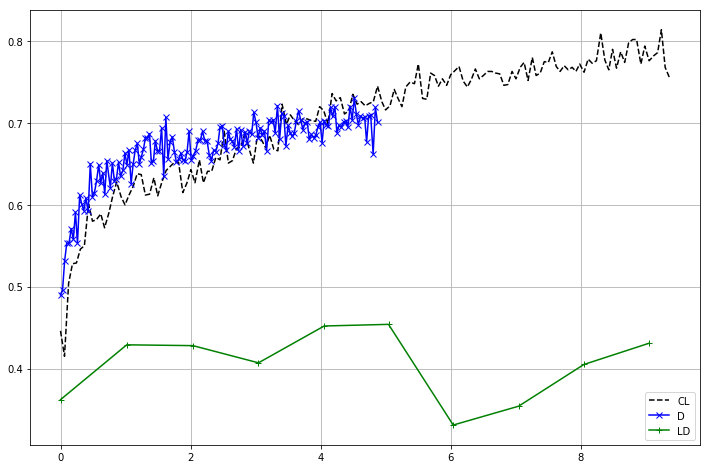
\includegraphics[width=0.65\textwidth]{content/random-block.png}
\caption{\label{fig:randomblock}Experiments with random blocks}%
\end{figure}
\todo[inline]{legenda}


%         \subsection{CL variations}
%         
Three variations of the ``CL'' network were made.
The ``CML'' network simply adds a max pooling layer to the convolutional layer.

The ``CLL'' network increases the output units of the convolutional layer and adds a LSTM layer with 64 output units before the final LSTM layer with 3 outputs. This change gives more parameters to the LSTM part of the network.

The ``CLD'' network also tries to increase the influence of the LSTM layer in the network. It reduces the convolutional input window while increases the number of output units. The number of output units of the LSTM network is increased to 128 and a fully connected layer is used as output layer.

The results of the experiments with these variations is shown in table \ref{tab:carvingclvariations}.
Overall, the ``CL'' network and this three variations produced similar results, as can be seen in figure \ref{fig:cl-variations}.

\begin{table}[!ht]
    \centering
    \caption{CL variations}
    \label{tab:carvingclvariations}
\begin{tabular}{r|r|r|r|r|r|r}
\hline
Name & Parameters & Blocks & Epochs & Time    & Training          & Validation          \\       
     &            &        &        &         &          accuracy &            accuracy \\ \hline\hline

CL & 24663  & all & 150 & 8m38s  & 0.813 & 0.783 \\ \hline
CLL & 287824  & all & 98  & 10m00s & 0.851 & 0.835 \\ \hline
CML & 262416  & all & 131 & 10m04s & 0.847 & 0.833 \\ \hline
CLD & 1246339 & all & 31  & 10m01s & 0.851 & 0.814 \\ \hline
\end{tabular}
\end{table}

\begin{figure}[htb!]
\centering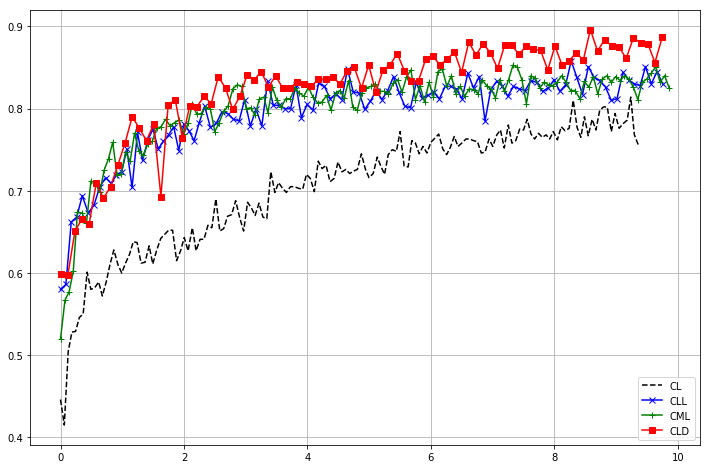
\includegraphics[width=0.65\textwidth]{content/cl-variations.png}
\caption{\label{fig:cl-variations}CL variations}%
\end{figure}
\todo[inline]{legenda}

%         \subsection{No LSTM}
%         To test if 
the LSTM layer could be replaced by 
another way of aggregating the convolutional layer outputs, three networks were constructed without any LSTM layer.

One of them, ``CM'' uses a stride of one and aggregates the results using a big max pooling layer.

Another one, ``CCM'' uses the same strategy, but includes another convolutional layer before the max pooling.

The last one, ``CD'', uses a bigger input window of 64 units, but with a smaller stride of 8 units. The output layer is a fully connected layer.

The results are shown in table \ref{tab:carvingnolstm}. The ``CL'' network is included for comparison.
These three networks produced similar results, but they are not as good as the ``CL'' network, as can be seen in figure
\ref{fig:nolstm}.


\begin{table}[!ht]
    \centering
    \caption{No LSTM}
    \label{tab:carvingnolstm}
\begin{tabular}{r|r|r|r|r|r|r}
\hline
Name & Parameters & Blocks & Epochs & Time & Training          & Validation          \\       
     &            &        &        &         &          accuracy &            accuracy \\ \hline\hline

CL & 24663  & all & 150 & 8m38s  & 0.813 & 0.783 \\ \hline
CM  & 24579   & all & 37 & 10m08s & 0.79  & 0.765 \\ \hline
CCM & 24600   & all & 36 & 10m13s & 0.764 & 0.732 \\ \hline
CD  & 1059587 & all & 47 & 10m11s & 0.745 & 0.739 \\ \hline
\end{tabular}
\end{table}

\begin{figure}[htb!]
\centering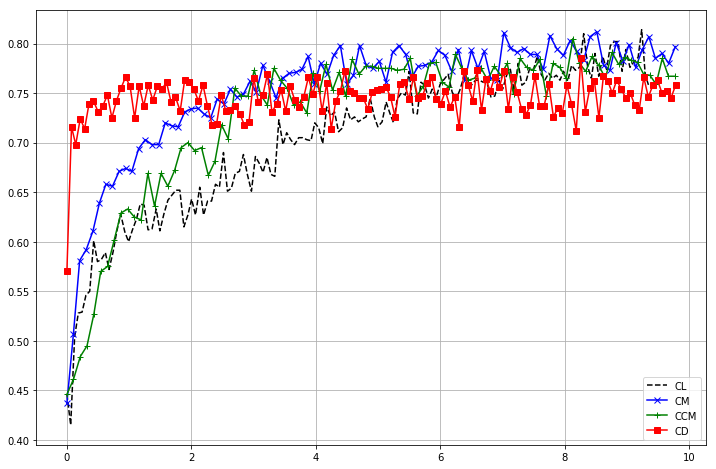
\includegraphics[width=0.65\textwidth]{content/nolstm.png}
\caption{\label{fig:nolstm}No LSTM}%
\end{figure}
\todo[inline]{legenda}


%         \subsection{Two convolutional layers}
%         To test if an increase on the deepness of the network would improve its results, four networks using two convolutional layers were experimented. 

At the ``CCL'' network, the first convolutional layer uses 8 units for the input window, and a stride of the same size, thus dividing the 512 bytes of the input block in 64 matrices of 8x256 that are then converted in 64 vectors of 128 units. The second layer divides the 64x128 input in 8 matrices of 8x128, producing 8 vectors of 64 units. The LSTM layer uses each of these 8 vectors as time steps, producing a single vector of 3 units, one for each class.

The ``CCLL'' network adds a LSTM layer of 64 output units between the convolutional layers and the final LSTM layer.

The ``CMCML'' network is similar to ``CCL'', but uses max pooling of size 2 at each convolutional layer.

The ``CMCMLL'' network combines the two additions, using max pooling and using two LSTM layers.

The results are shown in table \ref{tab:carving2convs}. The ``CL'' network is included for comparison. The ``CCL'' results were worst than ``CL'' ones, while ``CCLL'' were better. But the best results of all experiments described so far were those
These three networks produced similar results, but they are not as good as the ``CL'' network, as can be seen in figure
\ref{fig:nolstm}.

\begin{table}[!ht]
    \centering
    \caption{Two convolutional layers}
    \label{tab:carving2convs}
\begin{tabular}{r|r|r|r|r|r|r}
\hline
Name & Parameters & Blocks & Epochs & Time & Training          & Validation          \\       
     &            &        &        &         &          accuracy &            accuracy \\ \hline\hline

CL & 24663  & all & 150 & 8m38s  & 0.813 & 0.783 \\ \hline
CCL    & 328688 & all & 113 & 10m04s & 0.762 & 0.766 \\ \hline
CCLL   & 361712 & all & 98  & 10m02s & 0.853 & 0.823 \\ \hline
CMCML  & 295536 & all & 84  & 7m42s  & 0.902 & 0.858 \\ \hline
CMCMLL & 320752 & all & 94  & 10m01s & 0.887 & 0.871 \\ \hline
\end{tabular}
\end{table}

\begin{figure}[htb!]
\centering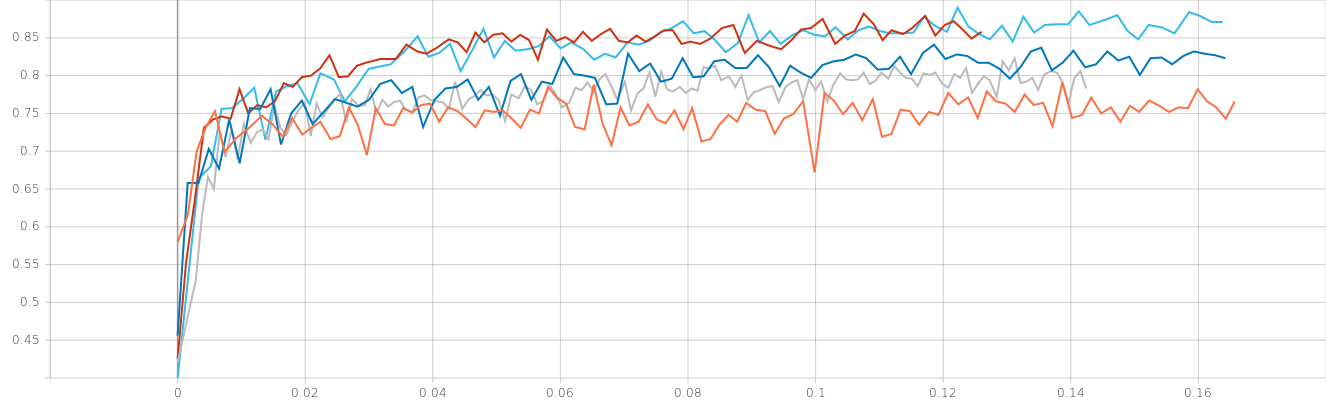
\includegraphics[width=0.65\textwidth]{content/twoconvs.png}
\caption{\label{fig:twoconvs}Two convolutional layers}%
\end{figure}
\todo[inline]{legenda}

%     \section{Discussion}
%     The best networks found among those examined in all set of experiments are the ``CMCML'' and ``CMCMLL''. Both have similar training times and final accuracy results, as their accuracy curves show. 

Table \ref{tab:carvinglayers} specify the number of output units in each layer of the networks used in the experiments. For the networks with two convolutional layers, those layers are connected together before the LSTM layer. For the convolutional layers, the input number indicates the size of the receptive field. 
\begin{table}[!ht]
    \centering
    \caption{Experiments layers}
    \label{tab:carvinglayers}
\begin{tabular}{r|r|r|r|r|r|r}

       & \multicolumn{4}{|c|}{}                         &        & Fully           \\     
       & \multicolumn{4}{|c|}{Convolutional}            & LSTM   &       connected \\ \hline
Name   & Input         & Stride & Output & Pooling size & Output & Output          \\ \hline\hline

D      &               &        &        &              &        & 3               \\ \hline
LD     &               &        &        &              & 32     & 3               \\ \hline
CL     & 32            & 32     & 3      &              & 3      &                 \\ \hline
CMCML  & 8             & 8      & 128    & 2            & 3      &                 \\       
       & 8             & 8      & 64     & 2            &        &                 \\ \hline
CMCMLL & 8             & 8      & 128    & 2            & 64     &                 \\       
       & 8             & 8      & 64     & 2            & 3      &                 \\ \hline
CLL    & 32            & 32     & 32     &              & 64     &                 \\       
       &               &        &        &              & 3      &                 \\ \hline
CML    & 32            & 32     & 32     & 2            & 3      &                 \\ \hline
CLD    & 16            & 16     & 256    &              & 128    & 3               \\ \hline
CD     & 64            & 8      & 64     &              &        & 3               \\ \hline
CM     & 32            & 1      & 3      & 481          &        &                 \\ \hline
CCM    & 32            & 1      & 3      &              &        &                 \\       
       & 2             & 2      & 3      & 240          &        &                 \\ \hline
\end{tabular}
\end{table}
% % \chapter{\label{chap:proposedsolution}Proposed solution}

% \todo[inline]{hypothesis on 2.1: amount of work}
% \todo[inline]{methodology (should be a chapter?)}

% % \chapter{\label{chap:validation}Validation}

% \chapter{\label{chap:conclusion}Conclusion}
% Among the examined networks, many satisfy the requirements imposed and could potentially be used by a forensic examiner to create a model to a new file type. This task could be done with little computational power, in a short time period and with a limited dataset. The networks that showed the best results are those that use convolutional layers to split and process the input and then use LSTM layers to analyse the series of outputs produced by the convolutional layers.
%     \section{Future work}
%     \begin{enumerate}[itemindent=\parindent,label=\textbf{Q\arabic*.}]

    \item Could a LSTM-based tool support a wider range of file types?
    
    \item Could a LSTM-based tool handle fragmentation through reassembling?
    
    \item Could a LSTM-based tool accept the addition of new file types by the end-user, in a collaborative manner? 


    \item Do the results obtained with usual datasets reflect what happens in real scenarios?

    \item Do LSTM neural networks help to interpret internal file structures?

\end{enumerate}
% \todo[inline]{compare solutions - possible candidates: feedforward, convolutional, LSTM, BLSTM, SVM, kNN, Photorec, Foremost, scalpel}
% \todo[inline]{shuffle data to simulate fragmentation}
% \todo[inline]{removal of portions of files to simulate data corruption}
% \todo[inline]{increase the number of supported file types, investigating the best strategy to scale the solution}
% \todo[inline]{reassembling}
% \todo[inline]{model share}
% \todo[inline]{adaption of visualization techniques of neural networks, attempting to infer file structure.}